\documentclass[11pt,a4paper,oneside]{report}             % Single-side
%\documentclass[11pt,a4paper,twoside,openright]{report}  % Duplex

%\PassOptionsToPackage{chapternumber=Huordinal}{magyar.ldf}
\usepackage{t1enc}
\usepackage[latin2]{inputenc}
\usepackage{amsmath}
\usepackage{amssymb}
\usepackage{enumerate}
\usepackage[thmmarks]{ntheorem}
\usepackage{graphics}
\usepackage{epsfig}
\usepackage{listings}
\usepackage{color}
%\usepackage{fancyhdr}
\usepackage{lastpage}
\usepackage{anysize}
\usepackage[magyar]{babel}
\usepackage{sectsty}
\usepackage{setspace}  % Ettol a tablazatok, abrak, labjegyzetek maradnak 1-es sorkozzel!
\usepackage[hang]{caption}
\usepackage{hyperref}
\usepackage[euler]{textgreek}
\usepackage[titletoc]{appendix}
% A paragraph form�z�shoz
\usepackage{titlesec}

% Paragraph form�z�s�nak fel�l�r�sa
\titleformat{\paragraph}
{\normalfont\normalsize\bfseries}{\theparagraph}{1em}{}
\titlespacing*{\paragraph}
{0pt}{3.25ex plus 1ex minus .2ex}{1.5ex plus .2ex}

%--------------------------------------------------------------------------------------
% Main variables
%--------------------------------------------------------------------------------------
\newcommand{\vikszerzo}{B�lint �d�m}
\newcommand{\vikkonzulens}{Szab� Zolt�n}
\newcommand{\cegkonzulens}{Mik� Gyula}
\newcommand{\vikcim}{Oper�ci�s rendszerek �sszehasonl�t�sa mikrovez�rl�s rendszerekben}
\newcommand{\viktanszek}{Automatiz�l�si �s Alkalmazott Informatikai Tansz�k}
\newcommand{\vikdoktipus}{Diplomaterv}
\newcommand{\vikdepartmentr}{B�lint �d�m}

%--------------------------------------------------------------------------------------
% Page layout setup
%--------------------------------------------------------------------------------------
% we need to redefine the pagestyle plain
% another possibility is to use the body of this command without \fancypagestyle
% and use \pagestyle{fancy} but in that case the special pages
% (like the ToC, the References, and the Chapter pages)remain in plane style

\pagestyle{plain}
%\setlength{\parindent}{0pt} % �ttekinthet�bb, angol nyelv� dokumentumokban jellemz�
%\setlength{\parskip}{8pt plus 3pt minus 3pt} % �ttekinthet�bb, angol nyelv� dokumentumokban jellemz�
\setlength{\parindent}{12pt} % magyar nyelv� dokumentumokban jellemz�
\setlength{\parskip}{0pt}    % magyar nyelv� dokumentumokban jellemz�

\marginsize{35mm}{25mm}{15mm}{15mm} % anysize package
\setcounter{secnumdepth}{0}
\sectionfont{\large\upshape\bfseries}
\setcounter{secnumdepth}{2}
\singlespacing
\frenchspacing

%--------------------------------------------------------------------------------------
%	Setup hyperref package
%--------------------------------------------------------------------------------------
\hypersetup{
    bookmarks=true,            % show bookmarks bar?
    unicode=false,             % non-Latin characters in Acrobat�s bookmarks
    pdftitle={\vikcim},        % title
    pdfauthor={\vikszerzo},    % author
    pdfsubject={\vikdoktipus}, % subject of the document
    pdfcreator={\vikszerzo},   % creator of the document
    pdfproducer={Producer},    % producer of the document
    pdfkeywords={keywords},    % list of keywords
    pdfnewwindow=true,         % links in new window
    colorlinks=true,           % false: boxed links; true: colored links
    linkcolor=black,           % color of internal links
    citecolor=black,           % color of links to bibliography
    filecolor=black,           % color of file links
    urlcolor=black             % color of external links
}

%--------------------------------------------------------------------------------------
% Set up listings
%--------------------------------------------------------------------------------------
\lstset{
	basicstyle=\scriptsize\ttfamily, % print whole listing small
	keywordstyle=\color{black}\bfseries\underbar, % underlined bold black keywords
	identifierstyle=, 					% nothing happens
	commentstyle=\color{white}, % white comments
	stringstyle=\scriptsize\sffamily, 			% typewriter type for strings
	showstringspaces=false,     % no special string spaces
	aboveskip=3pt,
	belowskip=3pt,
	columns=fixed,
	backgroundcolor=\color{lightgray},
} 		
\def\lstlistingname{lista}	

%--------------------------------------------------------------------------------------
%	Some new commands and declarations
%--------------------------------------------------------------------------------------
\newcommand{\code}[1]{{\upshape\ttfamily\scriptsize\indent #1}}

% define references
\newcommand{\figref}[1]{\ref{fig:#1}.}
\renewcommand{\eqref}[1]{(\ref{eq:#1})}
\newcommand{\listref}[1]{\ref{listing:#1}.}
\newcommand{\sectref}[1]{\ref{sect:#1}}
\newcommand{\tabref}[1]{\ref{tab:#1}.}

\DeclareMathOperator*{\argmax}{arg\,max}
%\DeclareMathOperator*[1]{\floor}{arg\,max}
\DeclareMathOperator{\sign}{sgn}
\DeclareMathOperator{\rot}{rot}
\definecolor{lightgray}{rgb}{0.95,0.95,0.95}

\author{\vikszerzo}
\title{\viktitle}
\includeonly{
	project,%
	titlepage,%
	declaration,%
	abstract,%
	introduction,%
	chapter1,%
	chapter2,%
	chapter3,%
	chapter4,%
	chapter5,%
	chapter6,%
	acknowledgement,%
	appendices,%
}
%--------------------------------------------------------------------------------------
%	Setup captions
%--------------------------------------------------------------------------------------
\captionsetup[figure]{
%labelsep=none,
%font={footnotesize,it},
%justification=justified,
width=.75\textwidth,
aboveskip=10pt}

\renewcommand{\captionlabelfont}{\small\bf}
\renewcommand{\captionfont}{\footnotesize\it}

%--------------------------------------------------------------------------------------
% Table of contents and the main text
%--------------------------------------------------------------------------------------
\begin{document}
\singlespacing
%--------------------------------------------------------------------------------------
% Feladatkiiras (a tanszeken atveheto, kinyomtatott valtozat)
%--------------------------------------------------------------------------------------
\clearpage
\begin{center}
\large
\textbf{FELADATKI�R�S}\\
\end{center}

A piaci term�kek el��ll�t�s�n�l gyakran a k�lts�gek k�tharmad�t a szoftverfejleszt�s teszi ki. Ez�rt a be�gyazott alkalmaz�sokn�l egyre ink�bb megszokott� v�lik be�gyazott oper�ci�s rendszerek haszn�lata. Az �sszetett hardverek alkalmaz�sa, a k�d �jrahasznos�that�s�ga, a csoportban t�rt�n� fejleszt�s �s a multitaszk ig�nye szint�n sz�ks�gess� teszi valamilyen oper�ci�s rendszer alkalmaz�s�t.


A feladat c�lja k�l�nb�z� oper�ci�s rendszerek megismer�se, el�nyeik �s h�tr�nyaik kitapasztal�sa �s egy ipari alkalmaz�son kereszt�l val� �sszehasonl�t�sa.
A hallgat� feladat�nak a k�vetkez�kre kell kiterjednie:
\begin{itemize}
	\item Adjon �ttekint�st az elterjedt oper�ci�s rendszerek
	\begin{itemize}
		\renewcommand\labelitemii{o}
		\item fel�p�t�s�r�l,
		\item m�k�d�s�r�l,
		\item el�nyeir�l,
		\item h�tr�nyair�l!
	\end{itemize}
	\item K�l�nb�z� fejleszt�k�rty�k seg�ts�g�vel hozzon l�tre be�gyazott oper�ci�s rendszeres alkalmaz�st!
	\item A feladat megold�sa sor�n haszn�ljon k�l�nb�z� komplexit�s� �s er�forr�s-ig�ny� oper�ci�s rendszereket!
	\item Hasonl�tsa �ssze az oper�ci�s rendszereket k�l�nb�z� szempontok alapj�n!
	\item A hallgat� v�gezzen irodalomkutat�st a teljes�tm�nymutat�k m�r�s�nek t�mak�r�ben!
	\item Tegyen javaslatot az �sszehasonl�t�s alapj�t ad� metrik�kra �s v�gezze el az �sszehasonl�t� teszteket!
	\item Adjon javaslatot az elemzett oper�ci�s rendszerek felhaszn�l�s�nak ter�leteire!
\end{itemize}

\pagenumbering{arabic}
\onehalfspacing
%--------------------------------------------------------------------------------------
%	The title page
%--------------------------------------------------------------------------------------
\begin{titlepage}
\begin{center}

\includegraphics[width=60mm,keepaspectratio]{figures/BMElogo.png}\\
\vspace{0.3cm}
\textbf{Budapesti M�szaki �s Gazdas�gtudom�nyi Egyetem}\\
\textmd{Villamosm�rn�ki �s Informatikai Kar}\\
\textmd{\viktanszek}\\[5cm]

\vspace{0.4cm}
{\huge \bfseries \vikcim}\\[0.8cm]
\vspace{0.5cm}
\textsc{\Large \vikdoktipus}\\[4cm]

\begin{tabular}{cc}
 \makebox[7cm]{\emph{K�sz�tette}} & \makebox[7cm]{\emph{Konzulens}} \\
 \makebox[7cm]{\vikszerzo} & \makebox[7cm]{\vikkonzulens}
\end{tabular}

\vfill
{\large \today}
\end{center}
\end{titlepage}



\tableofcontents\vfill
%--------------------------------------------------------------------------------------
% Nyilatkozat
%--------------------------------------------------------------------------------------
\begin{center}
\large
\textbf{HALLGAT�I NYILATKOZAT}\\
\end{center}

Alul�rott \emph{\vikszerzo}, szigorl� hallgat� kijelentem, hogy ezt a diplomatervet meg nem engedett seg�ts�g n�lk�l, saj�t magam k�sz�tettem, csak a megadott forr�sokat (szakirodalom, eszk�z�k stb.) haszn�ltam fel. Minden olyan r�szt, melyet sz� szerint, vagy azonos �rtelemben, de �tfogalmazva m�s forr�sb�l �tvettem, egy�rtelm�en, a forr�s megad�s�val megjel�ltem.

Hozz�j�rulok, hogy a jelen munk�m alapadatait (szerz�(k), c�m, angol �s magyar nyelv� tartalmi kivonat, k�sz�t�s �ve, konzulens(ek) neve) a BME VIK nyilv�nosan hozz�f�rhet� elektronikus form�ban, a munka teljes sz�veg�t pedig az egyetem bels� h�l�zat�n kereszt�l (vagy autentik�lt felhaszn�l�k sz�m�ra) k�zz�tegye. Kijelentem, hogy a beny�jtott munka �s annak elektronikus verzi�ja megegyezik. D�k�ni enged�llyel titkos�tott diplomatervek eset�n a dolgozat sz�vege csak 3 �v eltelte ut�n v�lik hozz�f�rhet�v�.

\begin{flushleft}
\vspace*{1cm}
Budapest, \today
\end{flushleft}

\begin{flushright}
 \vspace*{1cm}
 \makebox[7cm]{\rule{6cm}{.4pt}}\\
 \makebox[7cm]{\emph{\vikszerzo}}\\
 \makebox[7cm]{hallgat�}
\end{flushright}
\thispagestyle{empty}

\vfill
\clearpage
\thispagestyle{empty} % an empty page


%----------------------------------------------------------------------------
% Abstract in hungarian
%----------------------------------------------------------------------------
\chapter*{Kivonat}%\addcontentsline{toc}{chapter}{Kivonat}

Jelen dokumentum egy diplomaterv sablon, amely formai keretet ad a BME Villamosm�rn�ki �s Informatikai Kar�n v�gz� hallgat�k �ltal elk�sz�tend� szakdolgozatnak �s diplomatervnek. A sablon haszn�lata opcion�lis. Ez a sablon \LaTeX~alap�, a \emph{TeXLive} \TeX-implement�ci�val �s a PDF-\LaTeX~ford�t�val m�k�d�k�pes.
\vfill

%----------------------------------------------------------------------------
% Abstract in english
%----------------------------------------------------------------------------
\chapter*{Abstract}%\addcontentsline{toc}{chapter}{Abstract}

This document is a \LaTeX-based skeleton for BSc/MSc~theses of students at the Electrical Engineering and Informatics Faculty, Budapest University of Technology and Economics. The usage of this skeleton is optional. It has been tested with the \emph{TeXLive} \TeX~implementation, and it requires the PDF-\LaTeX~compiler.
\vfill


%----------------------------------------------------------------------------
\chapter*{Bevezet�}\addcontentsline{toc}{chapter}{Bevezet�}
%----------------------------------------------------------------------------

A bevezet� tartalmazza a diplomaterv-ki�r�s elemz�s�t, t�rt�nelmi el�zm�nyeit, a feladat indokolts�g�t (a motiv�ci� le�r�s�t), az eddigi megold�sokat, �s ennek t�kr�ben a hallgat� megold�s�nak �sszefoglal�s�t.

A bevezet� szok�s szerint a diplomaterv fel�p�t�s�vel z�r�dik, azaz annak r�vid le�r�s�val, hogy melyik fejezet mivel foglalkozik.


%----------------------------------------------------------------------------
\chapter{Elm�leti �ttekint�s}
%----------------------------------------------------------------------------

%----------------------------------------------------------------------------
\section{�ltal�nosan haszn�lt licencek}
%----------------------------------------------------------------------------

A mindennapi �letben naponta szembes�l�nk a k�l�nb�z� gy�rt�k vagy fejleszt�k �ltal el�rhet�v� tett programokkal, melyek mindegyike tartalmaz valamilyen megk�t�st a program haszn�lat�val kapcsolatban. Ezek k�z�tt tal�lhat�ak egyedileg alkalmazott felt�telek, de vannak elterjedt licencek, amiket p�ld�ul ny�lt forr�sk�d� szoftverek eset�n gyakran alkalmaznak.

%----------------------------------------------------------------------------
\subsection{Z�rt forr�sk�d� szoftver}
%----------------------------------------------------------------------------

Z�rt forr�sk�d� szoftver eset�n a forr�sk�d kiz�r�lag a gy�rt�/fejleszt� kez�ben marad. A szoftver haszn�lat��rt �ltal�ban valamekkora �sszeget kell fizetni, amely gyakran mag�ban foglalja a fell�p� probl�m�k megold�s�ban val� seg�ts�gny�jt�st is. 
Term�szetesen a z�rt forr�sk�d nem vonja k�telez�en maga ut�n, hogy a felhaszn�l�nak fizetnie kell a szoftver haszn�lat��rt. Sok gy�rt� a term�k�t ingyen el�rhet�v� teszi (freeware). Ilyen esetben a kereskedelmi c�l� felhaszn�l�sb�l �s/vagy a seg�ts�gny�jt�sb�l sz�rmazik a fejleszt�st fedez� bev�tel.
A gy�rt� a felhaszn�l�s felt�teleit saj�t maga szabhatja meg, �gy ebben az esetben nem lehet �ltal�nos elemz�st v�gezni a licencekkel kapcsolatban.

%----------------------------------------------------------------------------
\subsection{Ny�lt forr�sk�d� szoftver}
%----------------------------------------------------------------------------

A szoftverek m�sik nagy csoportj�t alkotj�k a ny�lt forr�sk�d� szoftverek. Ekkor a forr�sk�d publikusan el�rhet�. A ny�lt forr�sk�d� szoftverek eset�n is lehet�s�g van egy�ni licenc haszn�lat�ra, azonban a szoftverek t�bbs�g�n�l elterjedt, �ltal�nosan haszn�lt licencekkel tal�lkozunk.

%----------------------------------------------------------------------------
\subsubsection{MIT License}
%----------------------------------------------------------------------------

Az MIT licenc a legegyszer�bb licencek egyike. A licenc al� es� forr�sk�d szabadon m�solhat�, m�dos�that�, terjeszthet�, ak�r m�s licenc al� helyezhet�. 

%----------------------------------------------------------------------------
\subsubsection{Apache License 2.0}
%----------------------------------------------------------------------------

[ToDo]

%----------------------------------------------------------------------------
\subsubsection{BSD licenc}
%----------------------------------------------------------------------------

A BSD licenc eredetileg egy egyszer� �s szabad felfog�s� licenc sz�m�t�g�p szoftverek sz�m�ra, amit el�sz�r 1980-ban haszn�ltak a BSD UNIX oper�ci�s rendszerhez. Az id� el�rehaladt�val t�bb m�dos�t�st kellett v�grehajtani a licenc sz�vegez�s�n.

%----------------------------------------------------------------------------
\paragraph{4-clause BSD (eredeti)}
%----------------------------------------------------------------------------

Az eredeti, m�sn�ven 4-clause BSD licenc n�gy pontban foglalta �ssze a felhaszn�l�s felt�teleit. A licenc tartalmazza a szerz�i jog keletkez�s�nek �v�t, a fejleszt� szervezet nev�t �s a szerz�i jog tulajdonos�nak nev�t. A licenc megengedi a szoftver haszn�lat�t mind forr�s, mind bin�ris form�ban, ak�r m�dos�t�ssal, ak�r an�lk�l, amennyiben a felhaszn�l�s felt�telei teljes�lnek. A sz�veg azonban tartalmaz egy megk�t�st, amely a haszn�lat sor�n gyakran kellemetlens�gk�nt j�tt el� a felhaszn�l�k k�r�ben: amennyiben a szoftver b�rmilyen r�sz�re vagy a szoftver haszn�lat�ra hivatkoz�s t�rt�nik egy rekl�manyagban, �gy a szoftver fejleszt�j�t fel kellett t�ntetni a sz�vegben. Amennyiben t�bb, eredeti BSD licenc al� es� szoftvert tartalmaz� rendszer ker�lt hivatkoz�sra, �gy az eml�tett lista hamar nagy m�ret�v� v�lhatott. Ezen kellemetlens�g miatt ker�lt el�sz�r m�dos�t�sra a BSD licenc.

A n�gy pont az al�bbi felt�teleket szabja a feljhaszn�l� sz�m�ra:

\begin{enumerate}
\item A forr�sk�dnak tartalmaznia kell a copyright sz�veg�t, a felhaszn�l�s felt�teleit felsorakoztat� list�t, illetve a nyilatkozatot.
\item Bin�ris form�ban t�rt�n� terjeszt�s eset�n a copyright sz�veg�t, a felhaszn�l�s felt�teleit felsorakoztat� list�t, illetve a nyilatkoztatot a dokument�ci�ban �s/vagy valamely m�sik, a terjesztett szoftverhez adott anyagban fel kell t�ntetni.
\item B�rmif�le hirdet�si anyagban, ami a szoftver jellemz�ire vagy haszn�lat�ra hivatkozik, fel kell t�ntetnie az al�bbi elismer�st:
\emph{Ez a term�k a <szervezet> �ltal fejlesztett szoftvert tartalmaz.}
\item Sem a <szervezet> neve, sem a k�zrem�k�d� partneinek neve nem haszn�lhat� fel a szoftverb�l sz�rmaz� term�k n�pszer�s�t�s�re vagy aj�nl�s�ra erre vonatkoz� �r�sbeli enged�ly n�lk�l.
\end{enumerate}

A nyilatkozatban tiszt�z�sra ker�l, hogy a szerz�i jog tulajdonosa nem vonhat� felel�ss�gre a szoftver haszn�lat�b�l, felhaszn�l�s�b�l ered� �zemkimarad�s, adatveszt�s, profitveszt�s vagy egy�b vesztes�g bek�vetkez�se eset�n.

Ez a licencel�si forma ma m�r nem elterjedt, ink�bb a m�dos�tott (3-clause BSD) vagy az egyszer�s�tett (2-clause BSD) licenc haszn�lata aj�nlott.

%----------------------------------------------------------------------------
\paragraph{3-clause BSD (m�dos�tott)}
%----------------------------------------------------------------------------

Az el�z�, eredeti verzi�hoz k�pest a k�l�nbs�g, hogy elt�vol�tott�k a hirdet�sre vonatkoz� elismer�si felt�telt, valamint a nyilatkozat sz�veg�ben a k�zrem�k�d�ket is mentes�ti minden garanci�lis felel�ss�g al�l.

%----------------------------------------------------------------------------
\paragraph{2-clause BSD (egyszer�s�tett)}
%----------------------------------------------------------------------------

Az egyszer�s�tett (vagy gyakran FreeBSD licencnek is nevezett) BSD licenc k�t pontban foglalja �ssze a felhaszn�l�s felt�teleit, amit a m�dos�tott licencb�l a n�pszer�s�t�sre vonatkoz� pont elt�vol�t�s�val kaptak.

%----------------------------------------------------------------------------
\subsubsection{GNU GPL}
%----------------------------------------------------------------------------

A GNU General Public Licence azzal a c�llal j�tt l�tre, hogy garant�lja egy program szabad m�dos�t�s�t �s terjeszt�s�t, illetve hogy az szabad szoftver maradjon a felhaszn�l�i sz�m�ra. Az licenc az angol free kifejez�st nem a term�k �r�ra, hanem annak szabad felhaszn�l�s�ra haszn�lja.

A licenc t�bb m�dos�t�son kereszt�l ment. A k�t legutols� v�ltozatot ismertetem a tov�bbiakban.

%----------------------------------------------------------------------------
\paragraph{GNU GPLv2}
%----------------------------------------------------------------------------

A GNU GPLv2 licenc megengedi a program szabad terjeszt�s�t �s m�dos�t�s�t, amennyiben a terjesztett/m�dos�tott szoftver �r�kli az eredeti szerz�i jogi megjegyz�seket. A garanci�lis k�telezetts�gek elutas�t�sra ker�lnek, de nem tiltja meg (ak�r ellenszolg�ltat�s fej�ben) a v�llal�sukat. 

Ha m�dos�t�s t�rt�nt a programon, akkor fel kell t�ntetni a m�dos�t� nev�t �s a m�dos�t�s d�tum�t. 

A programt�l elk�l�n�thet� munk�ra nem k�telez� kiterjeszteni a licenc hat�ly�t, amennyiben az k�l�n ker�l terjeszt�sre. Ha az eredeti (szerz�i jogok al� es�) munk�val egy�tt ker�l terjeszt�sre, akkor automatikusan kiterjeszt�sre ker�lnek a felt�telek.

A program terjeszthet� futtathat�, bin�ris form�ban is, amennyiben a forr�sk�d publikusan el�rhet� marad.

A felhaszn�l� jogait tov�bb korl�tozni nem lehet.

Ha valamilyen okb�l kifoly�lag (p�ld�ul b�r�i v�gz�s folyt�n) a terjeszt�s csak bin�ris form�ban lehets�ges, akkor a program nem terjeszthet�.

Ha valamely orsz�gban a terjeszt�s nem lehets�ges, �gy a szerz�i jogok eredeti tulajdonosa f�ldrajzi megk�t�st adhat a terjeszt�sre vonatkoz�an, ami a licenc teljes �rt�k� r�sz�t k�pezi.

A programot m�s, szerz�i jogi szab�lyoz�s�ban k�l�nb�z� szoftverbe be�p�teni csak a szerz�t�l kapott enged�ly birtok�ban lehet.

A GPLv2 licenc nem engedi meg, hogy a program r�sze legyen szellemi tulajdont k�pez� szoftvernek. Ebben az esetben az LGPL licenc haszn�lata javasolt.

%----------------------------------------------------------------------------
\paragraph{GNU GPLv3}
%----------------------------------------------------------------------------

A GPL 2007-es m�dos�t�sa sor�n a tartalmi v�ltoztat�sokon k�v�l formai v�ltoztat�s is t�rt�nt, ami az �rthet�s�get hivatott szolg�lni. 

A tartalmi v�ltoztat�sok megc�lozz�k a m�s licencekkel val� kompatibilit�st, a licenccel v�dett szoftverhez j�r� felhaszn�l�i term�k m�dos�tott programmal val� haszn�lat�nak biztos�t�s�t (tivoiz�ci�\footnote{A TiVo egy digit�lis vide�r�gz�t� eszk�z�ket gy�rt� c�g, ami az eladott term�keiben GPLv2 licenc al� es� szoftverek haszn�lt. A Series~1 term�k�t m�dos�tott szoftverrel is lehetett haszn�lni, viszont a 2000-es �vek elej�n piacra dobott Series~2 DVR box-ban m�r digit�lis v�delmet haszn�ltak, ami megg�tolta a m�dos�tott rendszerek alkalmaz�s�t.} elker�l�se), jobban specifik�lja a jogok elveszt�s�t, illetve azok visszaszerz�s�nek lehet�s�geit, illetve megjelenik a \emph{megk�l�nb�ztet�} licenc defin�ci�ja. Megk�l�nb�ztet� licencnek tekintend� minden olyan licenc, ami nem tartalmazza az eredeti jogokat, vagy megtiltja valamely, az eredeti licencben foglalt jog gyakorl�s�t.

%----------------------------------------------------------------------------
\section{Oper�ci�s rendszer feladatai}
%----------------------------------------------------------------------------

Az oper�ci�s rendszer els�dleges feladata a haszn�lt processzor perif�ri�inak kezel�se, azokhoz meghat�rozott interf�sz biztos�t�sa. Tov�bbi feladata m�g a l�trehozott taszkok �temez�se, a taszkok k�z�tti kommunik�ci� �s szinkroniz�ci� megval�s�t�sa.

%----------------------------------------------------------------------------
\subsection{Oper�ci�s rendszer defin�ci�ja}
%----------------------------------------------------------------------------

Az oper�ci�s rendszer egy szoftver, ami kezeli a sz�m�t�g�p alap funkci�it �s szolg�ltat�sokat biztos�t m�s programok (vagy alkalmaz�sok) sz�m�ra. Az alkalmaz�sok val�s�tj�k meg azt a funkcionalit�st, amire a sz�m�t�g�p felhaszn�l�j�nak sz�ks�ge van, vagy a sz�m�t�g�p felhaszn�l�ja akar. Az oper�ci�s rendszer �ltal ny�jtott szolg�lat�sok az alkalmaz�sok fejleszt�s�t egyszer�s�tik, ez�ltal felgyors�tj�k a fejleszt�s folyamat�t �s karbantarthat�bb� teszik a szoftvert.

T�bbf�le oper�ci�s rendszert k�l�nb�ztet�nk meg a futtathat� folyamatok, az egyidej�leg kezelt felhaszn�l�k sz�m�nak �s az �temez� m�k�d�s�nek f�ggv�ny�ben. A tov�bbiakban csak a multitaszkot t�mogat� oper�ci�s rendszerekkel foglalkozom.

%----------------------------------------------------------------------------
\subsubsection{Val�sidej� oper�ci�s rendszer}
%----------------------------------------------------------------------------

A legt�bb oper�ci�s rendszer l�tsz�lag lehet�v� teszi t�bb program egyidej� futtat�s�t (multitasking). A val�s�gban minden processzor mag csak egy sz�lat tud egy id�pillanatban futtatni. Az oper�ci�s rendszer �temez�je a felel�s az�rt, hogy eld�ntse, melyik program mikor fusson, �s a programok k�zti gyors v�lt�ssal �ri el az egyidej� fut�s l�tszat�t (\figref{02_multitasking}a).

\begin{figure}[h!]
\center
\resizebox{13cm}{!}{
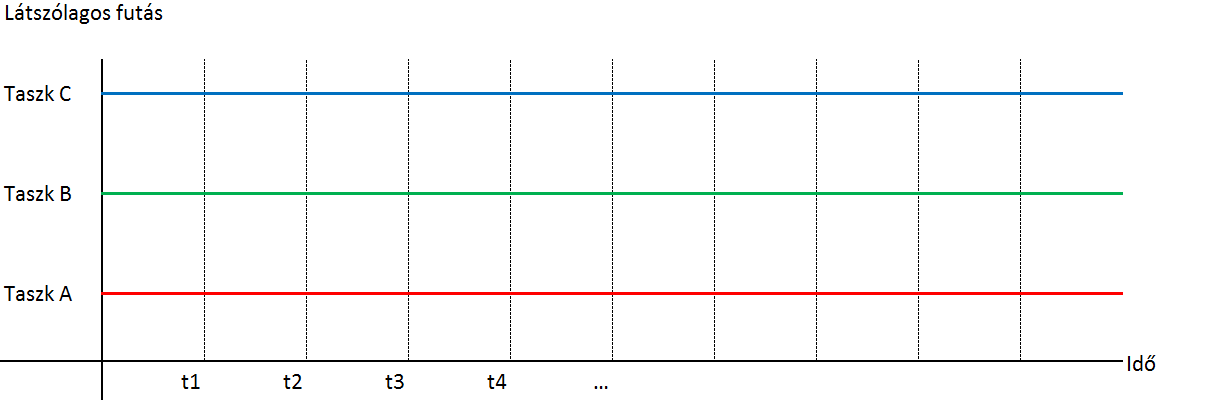
\includegraphics{figures/RTOS/01_parallel_run.png}}
\caption{L�tsz�lag a folyamatok p�rhuzamosan futnak.}
\label{fig:01_parallel_run}
\end{figure}

\begin{figure}[h!]
\center
\resizebox{13cm}{!}{
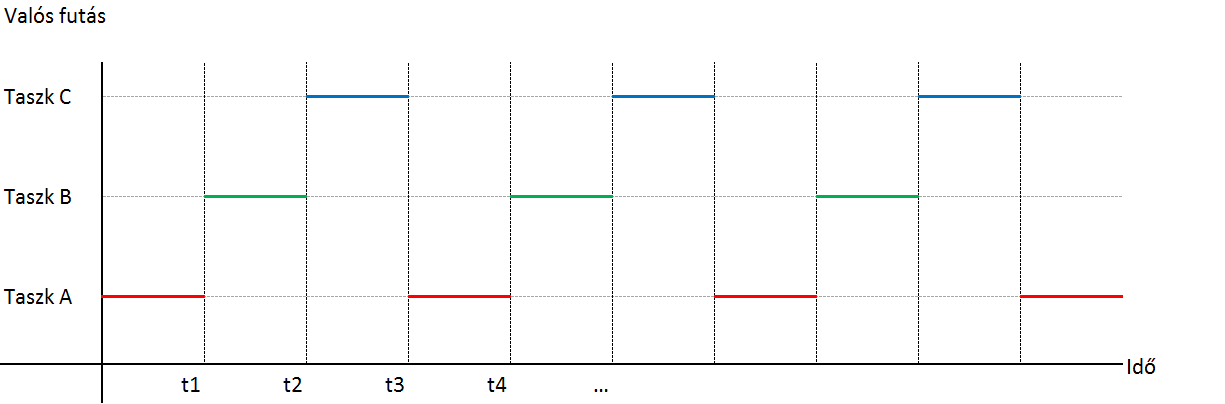
\includegraphics{figures/RTOS/02_multitasking.png}}
\caption{A val�s�gban minden folyamat egy kis id�szeletet kap a processzort�l.}
\label{fig:02_multitasking}
\end{figure}

Az oper�ci�s rendszer t�pus�t az �temez� d�nt�si mechanizmusa hat�rozza meg. Egy real-time oper�ci�s rendszer �temez�je �gy van megtervezve, hogy a v�grehajt�si minta determinisztikus legyen. Ez be�gyazott rendszerek eset�n �rdekes, mert a be�gyazott rendszerekn�l gyakran k�vetelm�ny a val�sidej�s�g, vagyis hogy a rendszernek egy szigor�an meghat�rozott id�n bel�l reag�lnia kell egy adott esem�nyre. A. val�sidej� k�vetelm�nyeknek val� megfelel�s csak �gy lehets�ges, ha az oper�ci�s rendszer �temez�je el�re megj�solhat� d�nt�seket hoz.

Val�sidej� oper�ci�s rendszerek k�z�l megk�l�nb�ztetj�k a soft real-time �s a hard real-time rendszereket.

Soft real-time rendszer eset�n nem probl�ma, ha nem �rkezik v�lasz a megadott hat�rid�n bel�l, az csak a rendszer min�s�t�s�t rontja.

Hard real-time rendszer eset�n viszont a rendszer alkalmatlann� v�lik a feladatra, ha a hat�rid�t nem tudja betartani. P�ld�ul egy szem�lyg�pj�rm� l�gzs�kj�nak k�sedelmes nyit�sa ak�r hal�los k�vetkezm�nyekkel is j�rhat.

%----------------------------------------------------------------------------
\subsection{�temez�s}
%----------------------------------------------------------------------------

Az oper�ci�s rendszer egyik meghat�roz� r�sze a haszn�lt �temez� m�k�d�s�nek elve, mely meghat�rozza az eszk�z alkalmass�g�t egy adott feladatra. Az �temez� d�nti el, hogy a fut�sra k�sz taszkok k�z�l melyik futhat a k�vetkez� �temez�si szakaszban. Tov�bbi feladata taszkv�lt�skor az �ppen fut� taszk �llapot�nak elment�se �s a futtatand� taszk �llapot�nak bet�lt�se. Az �temez� h�rom okb�l futhat le:
\begin{itemize}
\item Egy taszk lemond a fut�s jog�r�l,
\item Megszak�t�s �rkezik (tick esem�ny, k�ls� megszak�t�s),
\item Egy taszk l�trej�tt vagy befejez�d�tt.
\end{itemize}

A taszkv�lt�si m�d szerint k�tf�le m�k�d�st k�l�nb�ztet�nk meg:
\begin{description}
\item[$\bullet$\ Preempt�v �temez�s:] ekkor az �temez� megszak�thatja az �ppen fut� taszkot, amennyiben magasabb priorit�s� taszk fut�sra k�sz �llapotban v�rakozik,
\item[$\bullet$\ Nem-preempt�v vagy kooperat�v �temez�s:] ebben az esetben az �temez� csak akkor futtat �j taszkot, ha az �ppen fut� taszk befejez�d�tt vagy explicit lemond a fut�sr�l (blokkol�dik vagy �tadja a fut�s jog�t).
\end{description}

A tov�bbiakban ismertetem n�h�ny elterjedt �temez�si mechanizmus alapelv�t.

%----------------------------------------------------------------------------
\subsubsection{First-come first-served (Kiszolg�l�s be�rkez�si sorrendben)}
%----------------------------------------------------------------------------

A taszkok futtat�sa �rkez�si sorrendben t�rt�nik. A be�rkez� taszkok egy sorba ker�lnek, ahonnan sorrendben kapj�k meg a CPU haszn�lat jog�t.

Az �tlagos v�rakoz�si id� nagy lehet, ha egy id�ig�nyes folyamatra t�bb gyors lefut�s� folyamat v�rakozik.

Nem preempt�v.

%----------------------------------------------------------------------------
\subsubsection{Shortest Job First (Legr�videbb feladat el�sz�r)}
%----------------------------------------------------------------------------

A v�rhat�an leggyorsabban lefut� taszk ker�l fut�si �llapotba �temez�s bek�vetkez�sekor. Helyes m�k�d�s eset�n az �tlagos v�rakoz�si id� optim�lis lesz.

A gyakorlatban neh�z el�re megj�solni egy taszk fut�si idej�t.

Lehet preempt�v �s nem-preempt�v is. Preempt�v esetben Shortest Remaining Time First (Legr�videbb h�tralev� idej� el�sz�r) �temez�sr�l besz�l�nk.

%----------------------------------------------------------------------------
\subsubsection{Priorit�sos �temez�s}
%----------------------------------------------------------------------------

A k�vetkez� taszk kiv�laszt�sa a priorit�sa alapj�n t�rt�nik. N�velni lehet a hat�konys�g�t m�s met�dusok egyidej� haszn�lat�val (p�ld�ul a priorit�st a v�rhat� fut�si idej�b�l hat�rozzuk meg; a priorit�st n�velj�k az id� eltelt�vel; a priorit�st cs�kkentj�k az eddigi fut� �llapotban t�lt�tt id� ar�ny�ban).

Rossz tervez�s eset�n az alacsony priorit�s� feladatok nem jutnak processzorid�h�z (\mbox{ki�heztet�s}).

Lehet preempt�v �s nem-preempt�v is.

%----------------------------------------------------------------------------
\subsubsection{Round Robin}
%----------------------------------------------------------------------------

Id�oszt�son alapul� mechanizmus. A v�rakoz�si sor egy cirkul�ris buffer. Minden taszk adott id�szeletet kap, majd az id�szelet lej�rt�val a sorban k�vetkez� taszk kapja meg a fut�s jog�t.

%----------------------------------------------------------------------------
\subsubsection{Hibrid �temez�s}
%----------------------------------------------------------------------------

A felsorolt �temez�si elveket ak�r keverve is lehet alkalmazni. Ilyen �temez�si mechanizmus p�ld�ul a \emph{multilevel queue}, ahol minden sor saj�t �temez�si algoritmussal rendelkezik, �s egy k�l�n algoritmus felel az egyes sorok arbitr�ci�j��rt (\figref{05_multilevel_queue_scheduling}a).

\begin{figure}[h!]
\center
\resizebox{13cm}{!}{
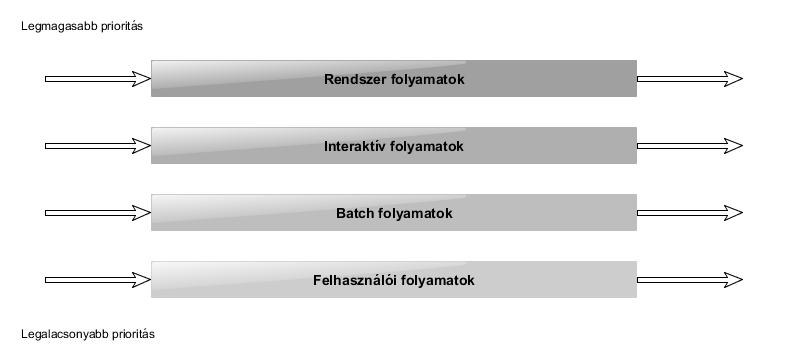
\includegraphics{figures/RTOS/05_multilevel_queue_scheduling.png}}
\caption{Multilevel queue �temez�s.}
\label{fig:05_multilevel_queue_scheduling}
\end{figure}

%----------------------------------------------------------------------------
\subsection{Oper�ci�s rendszer �ltal ny�jtott szolg�ltat�sok}
%----------------------------------------------------------------------------

Az oper�ci�s rendszer felel�s az egyes taszkoknak sz�ks�ges mem�riater�letek kezel�s��rt �s a taszkok k�z�tti kommunik�ci� megval�s�t�s��rt.

%----------------------------------------------------------------------------
\subsubsection{Mem�ria-kezel�s}
%----------------------------------------------------------------------------

Egy taszk l�trehoz�sakor az oper�ci�s rendszer osztja ki a taszk sz�m�ra a haszn�lhat� mem�riater�let hely�t �s m�ret�t, �s ezt az inform�ci�t a rendszernek t�rolnia kell. Ha az adott taszk befejezi a fut�s�t (megsz�nik), akkor az oper�ci�s rendszer feladata a taszkhoz tartoz� mem�riater�let felszabad�t�sa is.

 Amennyiben a taszk dinamikusan allok�l mem�ri�t fut�s k�zben, �gy ezen mem�ria kezel�se szint�n az oper�ci�s rendszer feladatk�r�be tartozik, viszont az egyszer�bb oper�ci�s rendszerek eset�ben a fut�s k�zben lefoglalt mem�ria felszabad�t�sa a taszk felel�s�ge.

%----------------------------------------------------------------------------
\subsubsection{Atomi m�velet}
%----------------------------------------------------------------------------

Bizonyos m�veletek sor�n sz�ks�g van a m�veletsor szigor�an egym�s ut�ni futtat�s�ra. Ilyen eset p�ld�ul a megosztott adatter�letre val� �r�s, amikor ha taszkv�lt�s k�vetkezik be az adatter�let �r�sa k�zben, akkor a tartalmazott adat �rv�nytelen �rt�ket vehet fel. Az ilyen, \emph{oszthatatlan} m�veleteket nevezz�k atomi m�veleteknek. 

A konzisztencia biztos�t�sa c�lj�b�l az atomi m�veleteket \emph{kritikus szakaszokba} kell �gyazni, ezzel jelezve az oper�ci�s rendszernek, hogy a m�veletek v�grehajt�sa alatt nem k�vetkezhet be taszkv�lt�s, bizonyos esetekben megszak�t�s sem.

Az oper�ci�s rendszerek a kritikus szakaszokat t�bb szinten megval�s�thatj�k. Legszigor�bb esetben a megszak�t�sok letilt�sra ker�lnek, �s az �temez� a kritikus szakasz befejez�s�ig felf�ggesztett �llapotban van. A kritikus szakasz megval�s�t�s�nak egy kev�sb� drasztikus m�dja az �temez� letilt�sa. Ekkor a k�dr�szlet v�dett a m�s taszkok �ltali preempt�l�st�l, viszont a megszak�t�sok nem ker�lnek letilt�sra.

A kritikus szakaszt a lehet� leggyorsabban el kell hagyni, mert k�l�nben a be�rkez� megszak�t�sok �s magasabb priorit�s� taszkok k�sleltet�st szenvednek, ami rontja az alkalmaz�s hat�konys�g�t.

%----------------------------------------------------------------------------
\subsubsection{Kommunik�ci�s objektumok}
%----------------------------------------------------------------------------

Az alkalmaz�sok egym�st�l f�ggetlen taszkok konstrukci�j�b�l �llnak. Viszont ezeknek a taszkoknak ahhoz, hogy a feladatukat el tudj�k l�tni, gyakran kommunik�lniuk kell egym�ssal.

A felsorolt kommunik�ci�s objektumok list�ja nem teljes. Bizonyos oper�ci�s rendszerek ezekt�l elt�r� strukt�r�kat is haszn�lhatnak, �s az itt felsorolt strukt�r�k implement�ci�ja is elt�rhet a le�rtakt�l (term�szetesen az sem biztos, hogy implement�lva van az adott objektum).

%----------------------------------------------------------------------------
\paragraph{Szemafor}
%----------------------------------------------------------------------------

K�t szemafor t�pust k�l�nb�ztet�nk meg:
\begin{itemize}
\item Bin�ris szemafor, amikor a szemafor k�t �rt�ket vehet fel,
\item Sz�ml�l� szemafor, mikor a szemafor t�bb �llapotot is felvehet.
\end{itemize}

A szemaforon k�t m�velet �rtelmezett:
\begin{itemize}
\item A szemafor jelz�se (elterjedt elnevez�sek: give, signal, post, V() m�velet\footnote{A jel�l�s a holland \emph{verhogen} (n�vel�s) sz�b�l sz�rmazik.}), amikor a szemafor �rt�ke n�vel�sre ker�l.
\item A szemafor elv�tele (elterjedt elnevez�sek: take, wait, pend, P() m�velet\footnote{A jel�l�s a holland \emph{proberen} (tesztel�s) sz�b�l sz�rmazik.}), amikor a szemafor el�sz�r tesztel�sre ker�l, hogy tartalmaz-e elemet, ha igen, akkor az �rt�k�t cs�kkentj�k, ha nem, akkor v�rakozunk addig, am�g valamelyik m�sik taszk el�rhet�v� nem teszi azt.
\end{itemize}

A szemafor l�tsz�lag egyszer�en helyettes�thet� egy egyszer� v�ltoz� (boolean vagy el�jel n�lk�li eg�sz) haszn�lat�val, viszont a be�p�tett szemafor strukt�ra atomi m�veletk�nt ker�l kezel�sre, illetve a rendszer automatikusan tudja kezelni a v�rakoz� folyamatok �llapotok k�zti mozgat�s�t.

Szemaforokat leggyakrabban szinkroniz�ci�s c�lb�l, vagy er�forr�sok v�delm�re haszn�lnak.

%----------------------------------------------------------------------------
\paragraph{Bin�ris szemafor}
%----------------------------------------------------------------------------

Bin�ris szemafor eset�n a szemafor k�t �rt�ket vehet fel. Felfoghat� �gy is, mint egy egy adat t�rol�s�ra alkalmas (egy elem hossz�) sor, melynek nem vizsg�ljuk a tartalmazott �rt�k�t, csak azt, hogy �ppen tartalmaz-e adatot vagy sem.

Leggyakoribb felhaszn�l�sa a taszkok szinkroniz�l�sa. Ekkor az egyik taszk a fut�s�nak egy adott pontj�n v�rakozik egy m�sik taszk jelz�s�re. Ezzel a m�dszerrel megval�s�that� a megszak�t�sok taszkokban t�rt�n� kezel�se, ezzel is minimaliz�lva a megszak�t�si rutin hossz�t. Erre l�thatunk p�ld�t \afigref{06_binary_semaphore}�n.

\begin{figure}[h!]
\center
\resizebox{8cm}{!}{
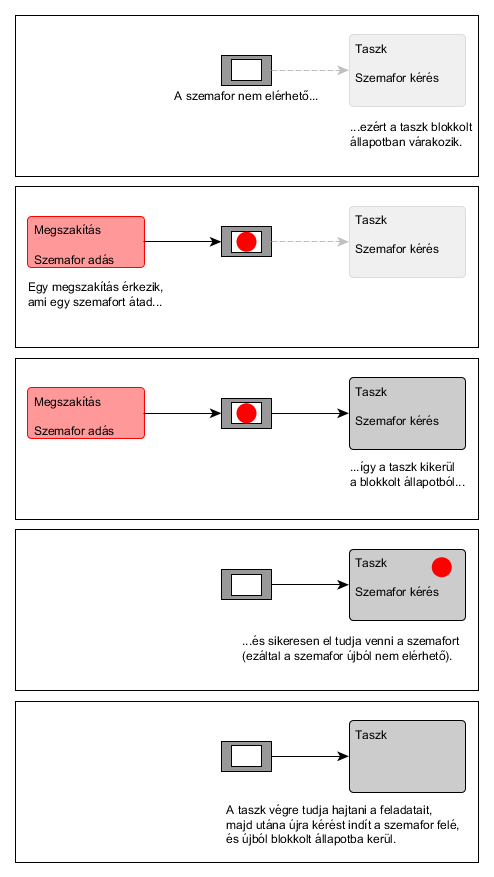
\includegraphics{figures/RTOS/06_binary_semaphore.png}}
\caption{Szinkroniz�ci� bin�ris szemafor seg�ts�g�vel.}
\label{fig:06_binary_semaphore}
\end{figure}

Bin�ris szemafor haszn�latakor k�l�n�s figyelmet kell ford�tani arra, hogy ha a szemafor egy adott taszkban gyakrabban ker�l jelz�sre, mint ahogy feldolgozzuk, akkor jelz�sek veszhetnek el. Am�g az egyik jelz�s v�rakozik, addig az ut�na k�vetkez� esem�nyeknek nincs lehet�s�g�k v�rakoz� �llapotba ker�lni (\figref{07_binary_semaphore_collision}a).

\begin{figure}[h!]
\center
\resizebox{8cm}{!}{
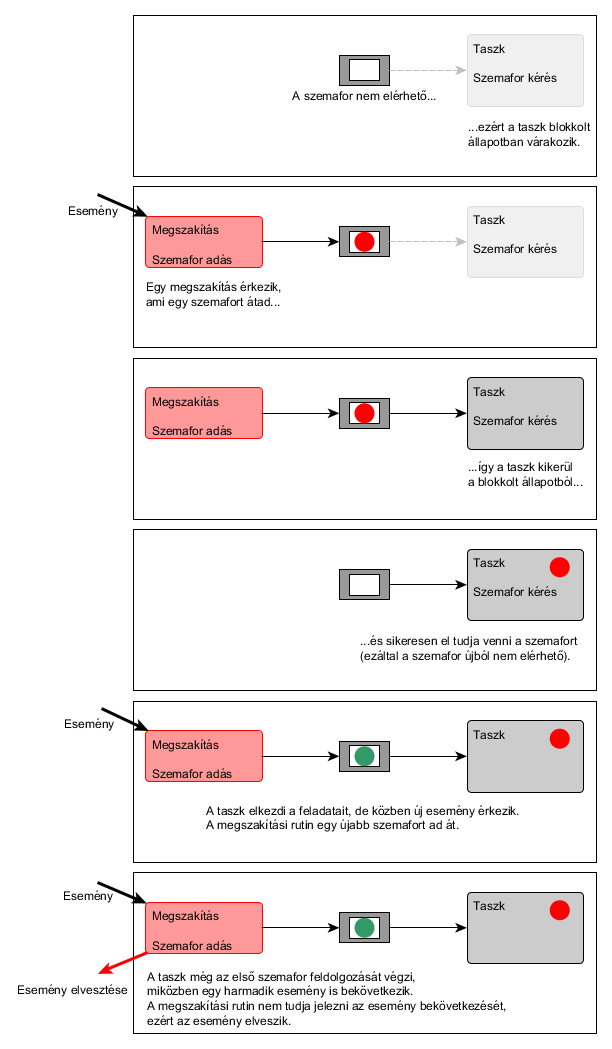
\includegraphics{figures/RTOS/07_binary_semaphore_collision.png}}
\caption{Esem�ny bek�vetkez�s�nek elveszt�se bin�ris szemafor haszn�lata sor�n.}
\label{fig:07_binary_semaphore_collision}
\end{figure}

%----------------------------------------------------------------------------
\paragraph{Sz�ml�l� szemafor}
%----------------------------------------------------------------------------

A sz�ml�l� t�pus� szemafor minden jelz�skor n�veli az �rt�k�t. Ekkor (am�g el nem �ri a maxim�lis �rt�k�t) nem ker�l \emph{Blokkolt} �llapotba a jelz� taszk. A sz�ml�l� szemafor felfoghat� �gy, mint egy egyn�l t�bb adat t�rol�s�ra k�pes sor (\figref{08_counting_semaphore}a), melynek nem vizsg�ljuk az �rt�k�t, csak azt, hogy �ppen tartalmaz-e m�g adatot vagy sem.

\begin{figure}[h!]
\center
\resizebox{8cm}{!}{
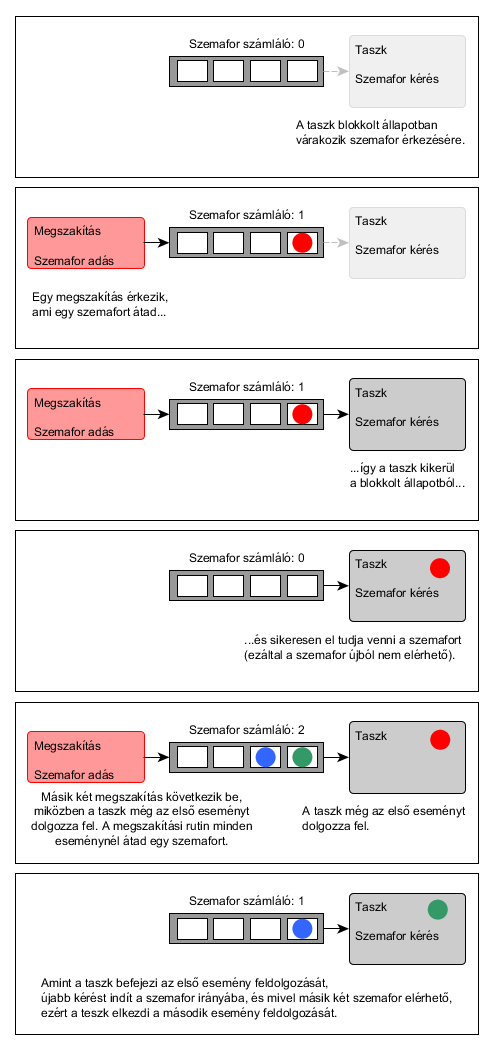
\includegraphics{figures/RTOS/08_counting_semaphore.png}}
\caption{Sz�ml�l� szemafor m�k�d�s�nek szeml�ltet�se.}
\label{fig:08_counting_semaphore}
\end{figure}

K�t felhaszn�l�sa elterjedt a sz�ml�l� szemaforoknak:
\begin{description}
\item[$\bullet$\ Esem�nyek sz�ml�l�sa:] ekkor minden esem�ny hat�s�ra n�velj�k a szemafor �rt�k�t (�j elemet helyez�nk a sorba). A szemafor aktu�lis �rt�ke a be�rkezett �s a feldolgozott esem�nyek k�l�nbs�ge. A sz�ml�l�sra haszn�lt szemafor inicializ�l�si �rt�ke nulla.
\item[$\bullet$\ Er�forr�s menedzsment:] ekkor a szemafor �rt�ke a rendelkez�sre �ll� er�forr�sok sz�m�t mutatja. Mikor az oper�ci�s rendszert�l az er�forr�st ig�nyelj�k, akkor a szemafor �rt�k�t cs�kkentj�k, mikor felszabad�tjuk a birtokolt er�forr�st, akkor a szemafor �rt�k�t n�velj�k. Ha a szemafor �rt�ke nulla, akkor nincs rendelkez�sre �ll� er�forr�s. Er�forr�sok kezel�s�re haszn�lt sz�ml�l� szemafor eset�n az inicializ�l�si �rt�k az el�rhet� er�forr�sok sz�ma.
\end{description}

%----------------------------------------------------------------------------
\paragraph{Mutex}
%----------------------------------------------------------------------------

Taszkok vagy taszkok �s megszak�t�si rutinok k�z�tt megosztott er�forr�s kezel�sekor a mutex (k�lcs�n�s kiz�r�s) haszn�lata indokolt. Mikor egy taszk vagy megszak�t�s hozz�f�r�st ind�t egy er�forr�shoz, akkor a hozz� tartoz� mutex-et elk�ri. Ha az er�forr�s szabad, akkor az ig�nyl� taszk megkapja a kezel�s jog�t, �s mindaddig megtartja, am�g be nem fejezi az er�forr�ssal val� munk�t (\figref{09_mutual_exclusion}a). A mutex-et a lehet� legkor�bban (az er�forr�ssal val� munka befejezt�vel) fel kell szabad�tani, ezzel is cs�kkentve az esetleges holtpont kialakul�s�nak vesz�ly�t. 

\begin{figure}[h!]
\center
\resizebox{8cm}{!}{
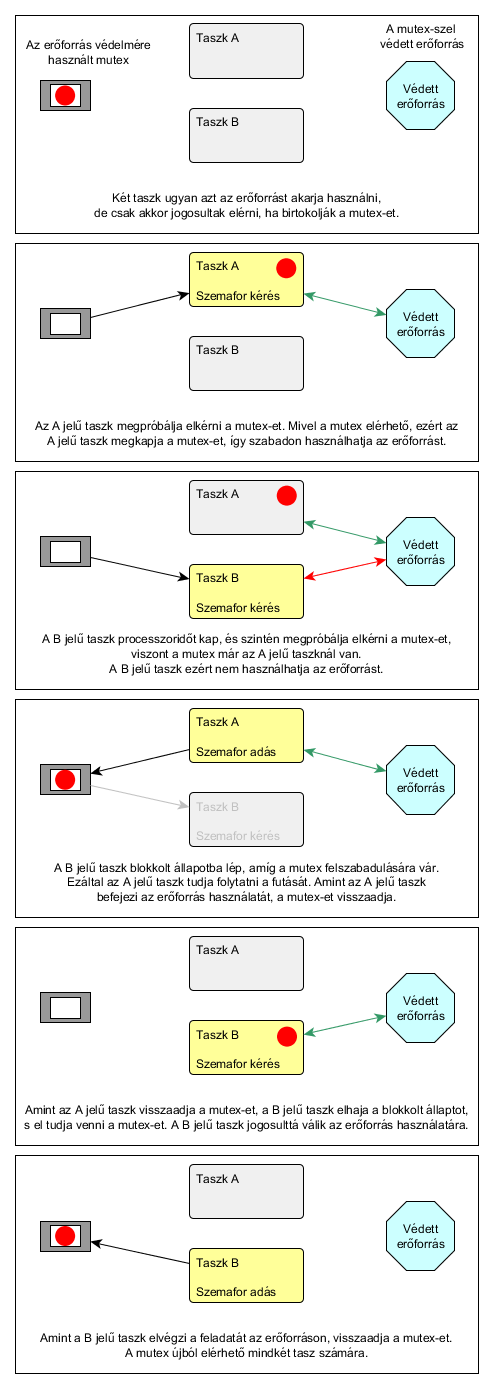
\includegraphics{figures/RTOS/09_mutual_exclusion.png}}
\caption{Mutex m�k�d�s�nek szeml�ltet�se.}
\label{fig:09_mutual_exclusion}
\end{figure}

L�that�, hogy a mutex nagyon hasonl�t a bin�ris szemaforhoz. A k�l�nbs�g abb�l ad�dik, hogy mivel a bin�ris szemafort leggyakrabban szinkroniz�ci�ra haszn�ljuk, ez�rt azt nem kell felszabad�tani: a jelz� taszk vagy megszak�t�s jelz�st ad a szemforon kereszt�l a feldolgoz� taszknak. A feldolgoz� taszk elveszi a szemafort, de a feldolgoz�s befejezt�vel a szemafort nem adja vissza. 

%----------------------------------------------------------------------------
\paragraph{Sor (Queue)}
%----------------------------------------------------------------------------

A sorok fix m�ret� adatb�l tudnak v�ges sz�m� �zenetet t�rolni. Ezek a jellemz�k a sor l�trehoz�sakor ker�lnek meghat�roz�sra. Alap�rtelmezetten FIFO-k�nt m�k�dik, aminek bemutat�s�t l�thatjuk \afigref{10_queue}�n.

\begin{figure}[h!]
\center
\resizebox{8cm}{!}{
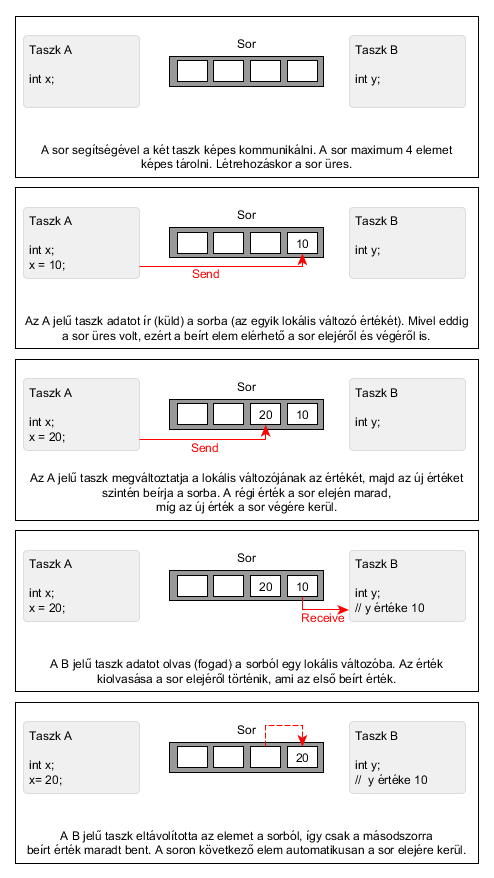
\includegraphics{figures/RTOS/10_queue.png}}
\caption{Sor m�k�d�s�nek szeml�ltet�se.}
\label{fig:10_queue}
\end{figure}

A sorba val� �r�s sor�n m�solat k�sz�l az eredeti v�ltoz�r�l, �s ez a m�solat ker�l t�rol�sra a sorban.

%----------------------------------------------------------------------------
\paragraph{�zenet (Message)}
%----------------------------------------------------------------------------

Az �zenet h�rom dolgot tartalmaz:
\begin{itemize}
\item Az adatra mutat� pointert,
\item A mutatott adat m�ret�t,
\item Egy id�b�lyegz�t, ami megmutatja, mikor ker�lt a pointer a t�rol�ba.
\end{itemize}

A pointer mutathat egy eg�sz adatter�letre vagy ak�r f�ggv�nyre is. A k�ld� �s fogad� f�lnek tudnia kell, hogy az �zenet tartalma mire mutat.

Mivel a kommunik�ci� sor�n csak az adat referenci�ja ker�l �tvitelre, ez�rt k�l�n�s figyelmet kell ford�tani az adat konzisztenci�j�ra.

%----------------------------------------------------------------------------
\paragraph{Esem�nyek (Event flag)}
%----------------------------------------------------------------------------

Az esem�nyek taszkok k�z�tti szinkroniz�ci�ra szolg�lnak. Megval�s�that� diszjunkt�v szinkroniz�ci�, amikor t�bb esem�ny k�z�l b�rmelyik bek�vetkez�se eset�n a taszk fut�sra k�sz �llapotba ker�l (logikai VAGY), �s megval�s�that� konjukt�v szinkroniz�ci�, amikor az esem�nyek mindegyik�nek bek�vetkez�se felt�tele a taszk fut�s�nak (logikai �S).

%----------------------------------------------------------------------------
\subsection{Oper�ci�s rendszer haszn�lata eset�n felmer�l� probl�m�k}
%----------------------------------------------------------------------------

Az alkalmaz�s �sszetetts�g�vel egy�tt n�vekszik a hib�k gyakoris�ga is. Oper�ci�s rendszer alkalmaz�sakor beleeshet�nk abba a hib�ba, hogy nem gondoljuk alaposan �t a szoftver m�k�d�s�t, ami k�l�nb�z� probl�m�k forr�sa lehet. A gyakran el�fordul�, tipikusnak tekinthet� probl�m�kra mutatok p�ld�kat a tov�bbiakban.

%----------------------------------------------------------------------------
\subsubsection{Ki�heztet�s (Starving)}
%----------------------------------------------------------------------------

Priorit�sos �temez�s eset�n, ha egy magas priorit�s� taszk folyamatosan fut�sra k�sz �llapotban van, akkor az alacsony priorit�s� taszkok sosem kapnak processzorid�t. Ezt a jelens�get nevezz�k ki�heztet�snek (starving), amit �tgondolt tervez�ssel k�nnyed�n elker�lhet�nk.

%----------------------------------------------------------------------------
\subsubsection{Priorit�s inverzi� (Priority inversion)}
%----------------------------------------------------------------------------

Vegy�nk egy esetet, mikor legal�bb h�rom, k�l�nb�z� priorit�si szinten fut� taszkot hozunk l�tre. A legalacsonyabb priorit�s�t�l a magasabb fel� haladva nevezz�k �ket \emph{TaskA}-nak, \emph{TaskB}-nek �s \emph{TaskC}-nek.

Kezdetben csak a \emph{TaskA} k�pes futni, ami egy mutex seg�ts�g�vel megkapja egy er�forr�s haszn�lati jog�t. K�zben a \emph{TaskC} fut�sra k�sz �llapotba ker�l, ez�rt preempt�lja a \emph{TaskA}-t. A \emph{TaskC} is haszn�ln� az er�forr�st, de mivel azt m�r a \emph{TaskA} birtokolja, ez�rt v�rakoz� �llapotba ker�l. K�zben a \emph{TaskB} is fut�sra k�sz �llapotba ker�lt, �s mivel magasabb a priorit�sa, mint a \emph{TaskA}-nak, ez�rt megkapja a fut�s jog�t. A \emph{TaskA} csak a \emph{TaskB} befejez�d�se (vagy blokkol�d�sa) eset�n ker�l �jra fut� �llapotba. Miut�n a \emph{TaskA} befejezte az er�forr�ssal a feladatait �s felszabad�tja azt, a \emph{TaskC} �jb�l fut�sra k�sz �llapotba ker�l, �s preempt�lja a \emph{TaskA}-t.

A magyar�zat illusztr�ci�ja \afigref{03_priority_inversion}�n l�that�.

\begin{figure}[h!]
\center
\resizebox{13cm}{!}{
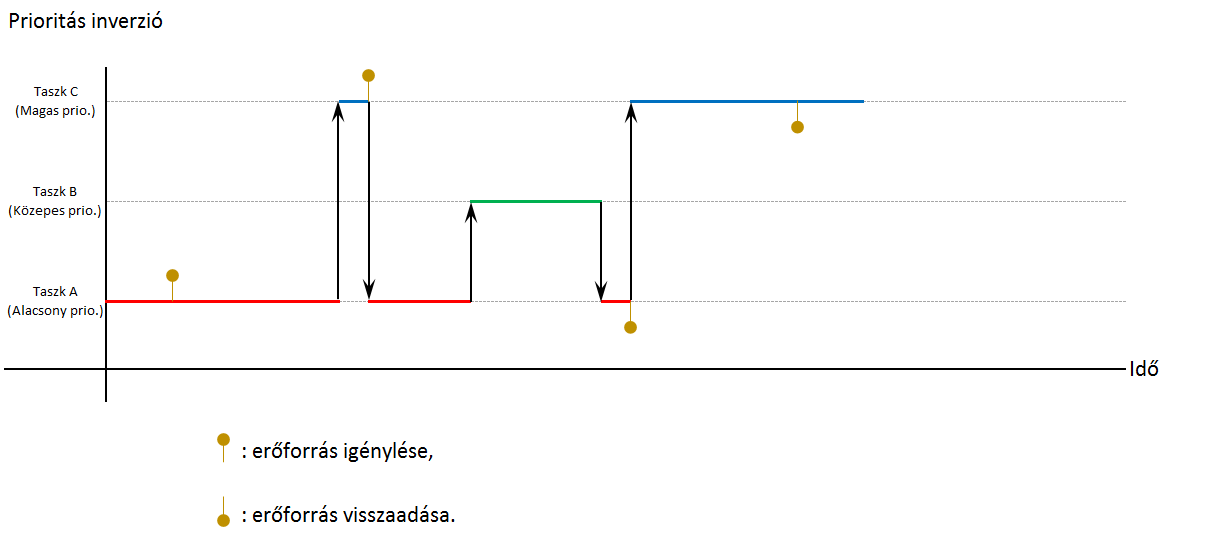
\includegraphics{figures/RTOS/03_priority_inversion.png}}
\caption{Priorit�s inverzi� jelens�ge.}
\label{fig:03_priority_inversion}
\end{figure}

A vizsg�lt p�lda sor�n a \emph{TaskB} k�sleltette a \emph{TaskC} fut�s�t azzal, hogy nem engedte a \emph{TaskA}-nak az er�forr�s felszabad�t�s�t. �gy l�tsz�lag a \emph{TaskB} magasabb priorit�ssal rendelkezett, mint \emph{TaskC}. Erre mondjuk, hogy priorit�s inverzi� l�pett fel.

A priorit�s inverzi� probl�m�j�nak egy megold�sa a priorit�s �r�kl�s. Ekkor a magas priorit�s� taszk a saj�t priorit�si szintj�re emeli azt az alacsony priorit�s� taszkot, mely blokkolja a tov�bbi fut�s�t (\figref{04_priority_inheritance}a). Amint a sz�ks�ges er�forr�s felszabadul, az eredeti priorit�si �rt�kek ker�lnek vissza�ll�t�sra.

\begin{figure}[h!]
\center
\resizebox{13cm}{!}{
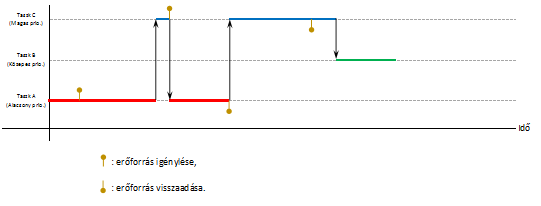
\includegraphics{figures/RTOS/04_priority_inheritance.png}}
\caption{Priorit�s �r�kl�s, mint a priorit�s inverzi� egyik megold�sa.}
\label{fig:04_priority_inheritance}
\end{figure}

%----------------------------------------------------------------------------
\subsubsection{Holtpont (Deadlock)}
%----------------------------------------------------------------------------

Szemaforok �s mutexek haszn�lata sor�n alakulhat ki holtponti helyzet. N�zz�k azt az esetet, hogy van k�t, azonos priorit�s� taszk (a taszkok priorit�sa itt nem l�nyeges), melyek m�k�d�s�k sor�n ugyan azt a k�t er�forr�st haszn�lj�k. A k�t taszkot nevezz�k \emph{TaskA}-nak �s \emph{TaskB}-nek, a k�t er�forr�st pedig \emph{ResA}-nak �s \emph{ResB}-nek (\figref{11_deadlock}a).

Indul�skor a \emph{TaskA} kapja meg a fut�s jog�t, �s lefoglalja a \emph{ResA}-t. K�zben lej�r a \emph{TaskA}-nak kiosztott id�szelet, �s \emph{TaskB} ker�l fut� �llapotba. A \emph{TaskB} lefoglalja a \emph{ResB} er�forr�st, majd megpr�b�lja lefoglalni a \emph{ResA} er�forr�st is. Mivel a \emph{ResA}-t m�r a \emph{TaskA} haszn�lja, ez�rt a \emph{TaskB} v�rakoz� �llapotba ker�l. A \emph{TaskA} �jb�l megkapja a processzort, �s hozz�f�r�st kezdem�nyez a \emph{ResB} er�forr�shoz. Mivel a \emph{ResB} er�forr�st a \emph{TaskB} folyamat birtokolja, ez�rt a \emph{TaskA} is v�rakoz� �llapotba l�p. Egyik folyamat sem tudja folytatni a feladat�t, emiatt az er�forr�sokat sem tudj�k felszabad�tani.

\begin{figure}[h!]
\center
\resizebox{8cm}{!}{
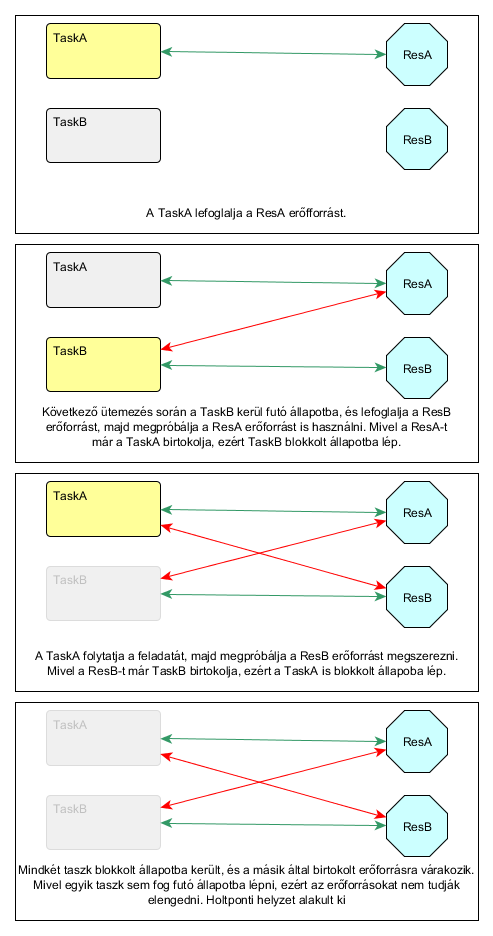
\includegraphics{figures/RTOS/11_deadlock.png}}
\caption{Holtponti helyzet kialakul�s�nak egy egyszer� p�ld�ja.}
\label{fig:11_deadlock}
\end{figure}

A holtponti helyzetek elker�l�s�re �s felold�s�ra t�bb szab�ly l�tezik, de be�gyazott rendszerekn�l �tgondolt tervez�ssel, illetve id�korl�t megad�s�val �ltal�ban elker�lhet� a kialakul�suk.

%----------------------------------------------------------------------------
\subsubsection{�jrah�vhat� f�ggv�nyek (Reentrant functions)}
%----------------------------------------------------------------------------

Egy f�ggv�ny reentr�ns (�jrah�vhat�), ha biztons�gosan megh�vhat� t�bb k�l�nb�z� taszkb�l vagy megszak�t�sb�l.

Minden taszk rendelkezik saj�t stack-kel �s saj�t regiszterekkel. Ha egy f�ggv�ny minden adatot a stack-j�n vagy a regisztereiben t�rol (vagyis nem haszn�l glob�lis �s statikus v�ltoz�kat), akkor a f�ggv�ny reentr�ns.
%----------------------------------------------------------------------------
\chapter{Oper�ci�s rendszerek bemutat�sa}
%----------------------------------------------------------------------------

%----------------------------------------------------------------------------
\section{Haszn�lt fejleszt�k�rty�k}
%----------------------------------------------------------------------------

%----------------------------------------------------------------------------
\subsection{STM32F4~Discovery}
%----------------------------------------------------------------------------

Manaps�g egyre ink�bb teret nyernek maguknak az ARM alap� mikrokontrollerek, melyek nem csak nagy sz�m�t�si kapacit�sukkal, de egyre alacsonyabb �rukkal szor�tj�k ki versenyt�rsaikat. Az egyik legelterjedtebb gy�rt�, az STMicroelectronics (tov�bbiakban STM) t�bb fejleszt�k�rty�t is piacra bocs�tott az elm�lt �vekben, melyeken k�l�nb�z� mikrokontrollerek k�pess�geit ismerheti meg a fejleszt�. A kaphat� fejleszt�k�rty�k amellett, hogy megk�m�lik a fejleszt�t a saj�t hardver tervez�s�t�l -- �gy a tervez�si hib�b�l ad�d� probl�m�k keres�s�t�l is --, a legt�bb esetben a gy�rt� sz�les k�r� t�mogat�st is ny�jt a term�kekhez (mintaprogramok, f�rumok, stb.).

Az STM �ltal gy�rtott fejleszt�k�rty�k k�z�l �r-�rt�k ar�ny�nak k�sz�nhet�en tal�n a leggyakrabban haszn�lt az STM32F407 Discovery (tov�bbiakban STM32F4 Discovery) k�rtya. A rajta tal�lhat� mikrokontroller rendelkezik a legt�bb alkalmaz�sban el�fordul� perif�ri�k mindegyik�vel. A teljess�g ig�nye n�lk�l:

\begin{itemize}
\item GPIO-k,
\item Soros kommunik�ci�s portok (szinkron �s aszinkron egyar�nt),
\item Ethernet port,
\item Analog-Digital Converter,
\item Digital-Analog Converter,
\item Id�z�t�k,
\item High-Speed~USB (OTG t�mogat�ssal),
\item SPI,
\item I$^\textrm{2}$C,
\item I$^\textrm{2}$S,
\item SDIO (SD illetve MMC k�rtya kezel�s�hez),
\item CAN,
\item Szoftveres �s hardveres magszak�t�sok.
\end{itemize}

A nagysz�m� perif�ria mellett a mikrokontroller sz�m�t�si kapacit�sa is kimagaslik a hasonl� �rkateg�ri�j� eszk�z�k k�r�b�l, k�sz�nhet�en az ak�r 168~MHz-es �rajel�nek, a be�p�tett CRC �s lebeg� pontos aritmetikai egys�g�nek, illetve a t�bb perif�ri�t is kezelni k�pes DMA-knak.

Az eszk�z 1~MByte Flash mem�ri�val �s 192~kbyte RAM-mal rendelkezik\cite{STMRef}.

A k�rty�n megtal�lhat� t�bb perif�ria, mely a k�l�nb�z� interf�szek kipr�b�l�s�t teszi lehet�v� (mint p�ld�ul gyorsul�sszenzor, mikrofon).

\begin{figure}[h!]
\center
\resizebox{8cm}{!}{
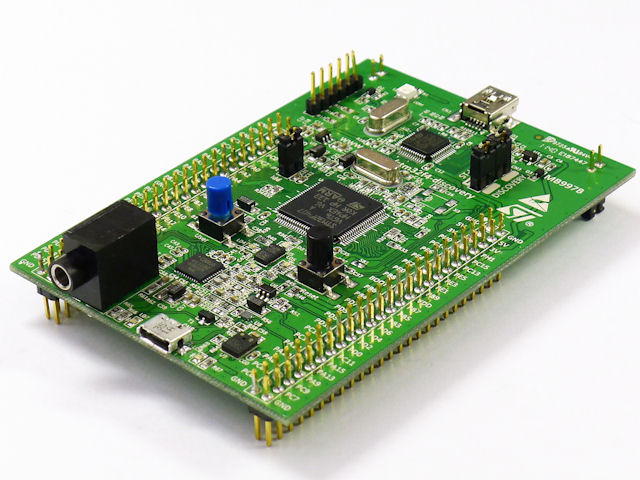
\includegraphics{figures/Eval_Boards/01_STM32F4-Discovery.jpg}}
\caption{STM32F4 Discovery fejleszt�k�rtya.}
\label{fig:01_STM32F4-Discovery}
\end{figure}


\subsubsection{STM32F4 Discovery - Base Board}

Az STM32F4 Discovery fejleszt�eszk�zh�z t�bb kieg�sz�t� k�rtya is kaphat�, melyek c�lja a kipr�b�lhat� perif�ri�k sz�m�nak n�vel�se. Egyik ilyen b�v�t�k�rtya az STM32F4DIS-BB, ami tartalmaz microSD-k�rtya foglalatot, az Ethernet interf�sz fizikai r�teg�t megval�s�t� IC-t, illetve a csatlakoztat�shoz sz�ks�ges RJ45-�s csatlakoz�t. Ezen k�v�l tal�lhat� rajta egy DB9-es csatlakoz� -- mely az egyik soros kommunik�ci�s portot teszi el�rhet�v� --, egy FPC csatlakoz� -- mely kamera csatlakoztat�s�t teszi lehet�v� --, illetve az egyik oldali csatlakoz�sorra r�k�thet� 3,5~"-os TFT kijelz�.

\begin{figure}[h!]
\center
\resizebox{8cm}{!}{
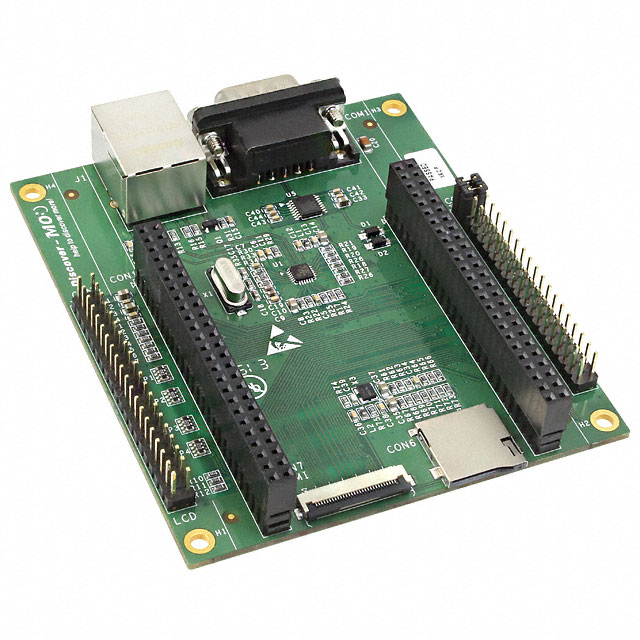
\includegraphics{figures/Eval_Boards/02_STM32F4DIS-BB.jpg}}
\caption{STM32F4 Discovery BaseBoard kieg�sz�t� k�rtya.}
\label{fig:02_STM32F4DIS-BB}
\end{figure}

%----------------------------------------------------------------------------
\subsection{Raspberry~Pi~3}
%----------------------------------------------------------------------------

A Raspberry Pi Foundation-t 2008-ban alap�tott�k azzal a c�llal, hogy a informatikai tudom�nyok ter�let�n seg�tse az oktat�st\cite{RaspiHistory}.

Az els� nagyteljes�tm�ny�, bankk�rtya m�ret� sz�m�t�g�p�ket 2012 febru�rj�ban bocs�tott�k piacra, melynek �ra t�red�ke volt az asztali sz�m�t�g�pek�nek. Az�ta t�bb verzi�ja is megjelent az eszk�znek, melyet folyamatosan fejlesztettek mind teljes�tm�nyben, mind az integr�lt funkci�k sz�m�ban. 2015 november�ben a vil�g els� 5\,\$-os sz�m�t�g�p�vel jelentek meg a piacon, melynek a Raspberry~Pi~Zero nevet adt�k\cite{RaspiHistory}.

A leg�jabb verzi�j� k�rtya, a Raspberry Pi 3 model B az el�z� verzi�hoz k�pest er�sebb processzort kapott, illetve tartalmaz be�p�tett Bluetooth illetve WiFi modult.

\begin{figure}[h!]
\center
\resizebox{8cm}{!}{
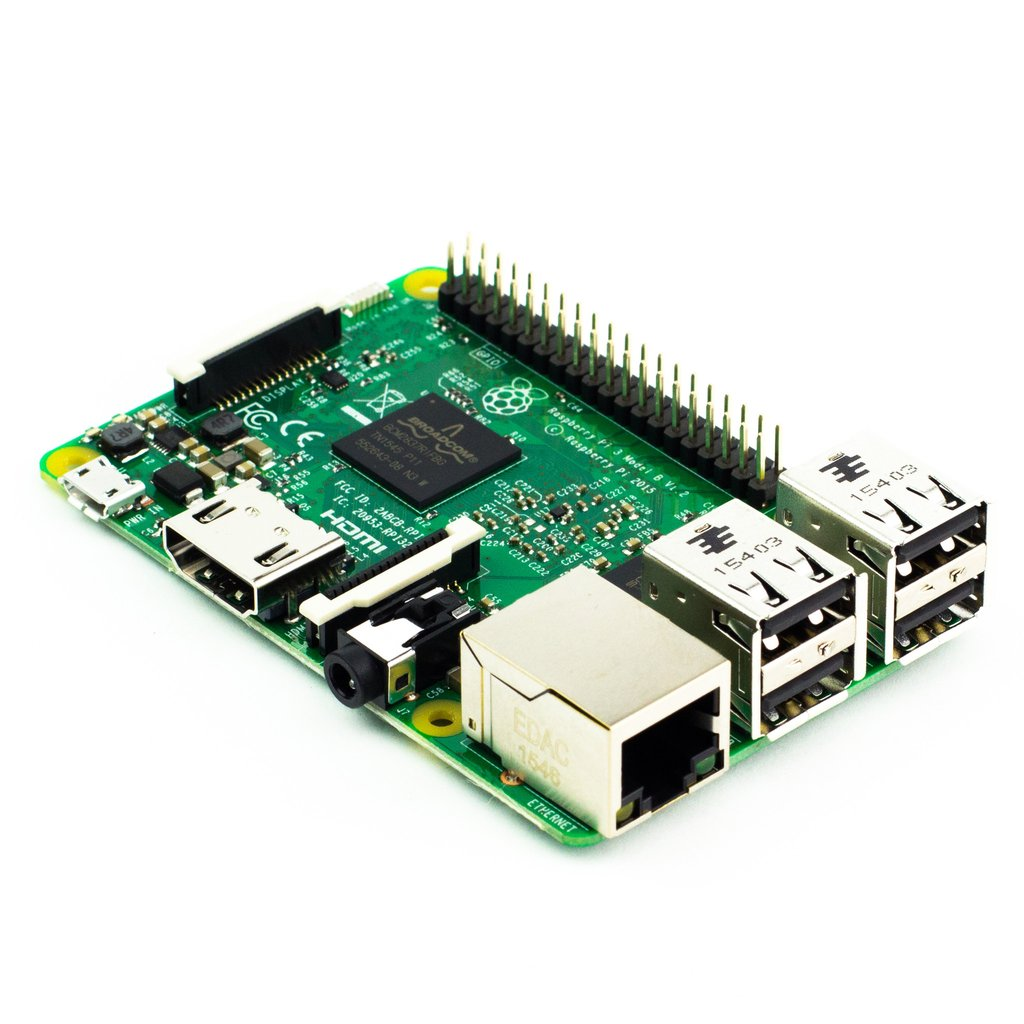
\includegraphics{figures/Eval_Boards/03_Raspberry_Pi_3.jpg}}
\caption{Raspberry~Pi~3 bankk�rtya m�ret� PC.}
\label{fig:03_Raspberry_Pi_3-BB}
\end{figure}

A hardver f�bb jellemz�i:
\begin{itemize}
\item 1,2~GHz 64-bit quad-core ARMv8 CPU,
\item 802.11n Wireless LAN,
\item Bluetooth 4.1,
\item Bluetooth Low Energy,
\item 1~GB RAM,
\item 4 USB port,
\item 40 GPIO pin,
\item HDMI port,
\item Ethernet port,
\item Kombin�lt 3,5~mm-es jack aljzat (audio �s kompozit vide�),
\item MicroSD k�rtyafoglalat,
\item VideoCore IV GPU.
\end{itemize}

Interf�szek:
\begin{itemize}
\item SPI,
\item UART,
\item DPI (Display Parallel Interface),
\item SDIO,
\item PCM (Pulse-code Modulation),
\item 1-WIRE,
\item JTAG,
\item GPCLK (General Purpose Clock),
\item PWM.
\end{itemize}

M�r az els� verzi� megjelen�sekor rendelkez�sre �lltak k�l�nb�z� linux disztrib�ci�k portjai, melyekkel az eszk�z asztali sz�m�t�g�pk�nt haszn�lhat� volt. N�pszer�s�g�nek k�sz�nhet�en a m�sodik verzi�t�l kezdve m�r a Windows~10~IoT~Core is t�mogatja a platformot.

%----------------------------------------------------------------------------
\section{A v�laszt�s szempontjai}
%----------------------------------------------------------------------------

Az oper�ci�s rendszerek kiv�laszt�s�n�l els�dleges szempont a hardverek t�mogatotts�ga, illetve az oktat�si c�lra val� el�rhet�s�g volt.

%----------------------------------------------------------------------------
\subsection{STM32F4~Discovery}
%----------------------------------------------------------------------------

Az UBM Tech minden �vben k�sz�t kutat�st a be�gyazott rendszereket piac�n, melyben t�bbek k�z�tt a haszn�lt be�gyazott oper�ci�s rendszerekkel kapcsolatban is publik�l adatokat (a 2015-�s felm�r�s eredm�nye l�that� \afigref{01_OS_popularity}�n). A statisztika alapj�n a k�t leggyakrabban haszn�lt oper�ci�s rendszer a \mbox{FreeRTOS} �s a \mbox{\textmugreek C/OS--II}. A \textmugreek C/OS �j verzi�ja, a \mbox{\textmugreek C/OS--III} a list�n h�tr�bb kapott helyet, de m�g �gy is bef�rt a t�z vezet� rendszer k�z�. Mindh�rom oper�ci�s rendszer n�pszer�s�ge n�tt a 2014-es �vhez k�pest.

\begin{figure}[h!]
\center
\resizebox{15cm}{!}{
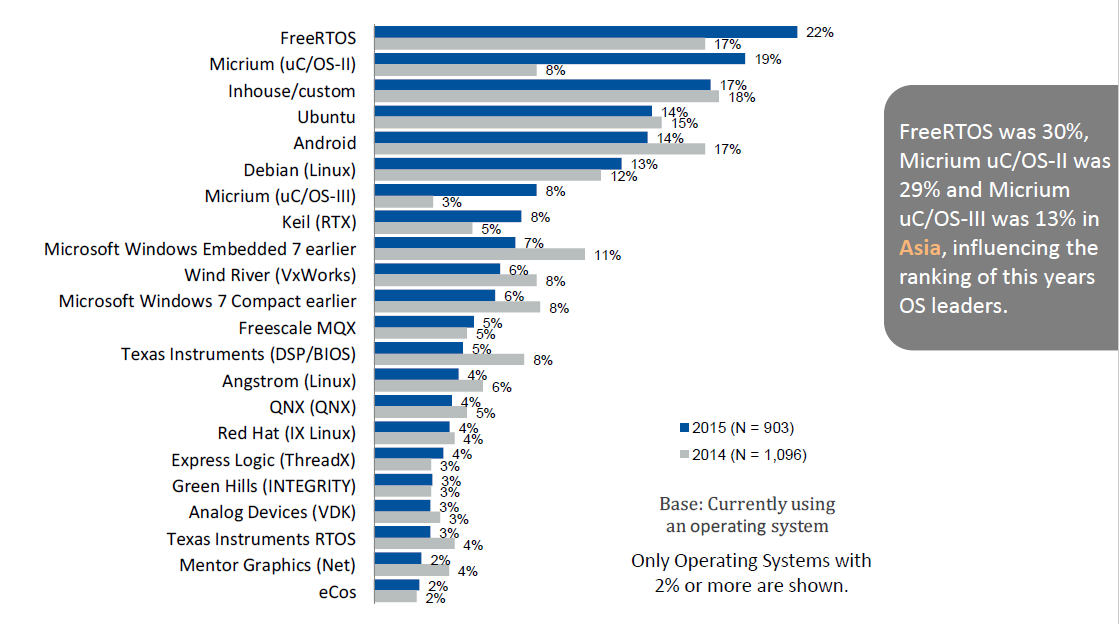
\includegraphics{figures/OS_selection/01_OS_popularity.png}}
\caption{Az UBM~Tech �ltal 2015-ben publik�lt be�gyazott oper�ci�s rendszer haszn�lati statisztika\cite{UBMStudy}.}
\label{fig:01_OS_popularity}
\end{figure}

Az STM32F4 Discovery k�rty�hoz el�rhet� szoftvercsomag tartalmazza a \mbox{FreeRTOS} rendszert, ami jelzi a rendszer t�mogatotts�g�nak m�rt�k�t. A \mbox{FreeRTOS} hivatalos oldal�n megv�s�rolhat�ak a rendszer haszn�lat�t bemutat� k�nyvek, illetve online el�rhet�ek le�r�sok, amik szint�n seg�tik a rendszer megismer�s�t. Ez�ltal az els� megvizsg�lt rendszernek a \mbox{FreeRTOS}-t v�lasztottam.

A Micrium \textmugreek C/OS rendszerei oktat�si c�lra ingyenesen el�rhet�ek, bele�rtve a rendszer dokument�ci�it is. A v�lasztott m�sik rendszer a \mbox{\textmugreek C/OS--III}.

%----------------------------------------------------------------------------
\subsection{Raspberry~Pi~3}
%----------------------------------------------------------------------------

A Raspberry Pi megjelen�se �ta t�mogatja k�l�nb�z� linux disztrib�ci�k futtat�s�t az eszk�z�n, �s a fejleszt�k�rtya m�sodik verzi�ja �ta a Windows 10 IoT Core is telep�thet� r�. Az asztali alkalmaz�s fejleszt�k k�r�ben mind a linux, mind a Windows elterjedten haszn�lt oper�ci�s rendszer, ez�rt a Raspberry Pi 3-on ezt a k�t rendszert vizsg�lom meg.

%----------------------------------------------------------------------------
\input{FreeRTOS}
%----------------------------------------------------------------------------

%----------------------------------------------------------------------------
%----------------------------------------------------------------------------
\section{\textmugreek C/OS-III}
%----------------------------------------------------------------------------
%----------------------------------------------------------------------------

%----------------------------------------------------------------------------
%----------------------------------------------------------------------------
\section{Linux}
%----------------------------------------------------------------------------
%----------------------------------------------------------------------------

%----------------------------------------------------------------------------
%----------------------------------------------------------------------------
\section{Windows 10 IoT Core}
%----------------------------------------------------------------------------

A Windows~10~IoT~Core a Windows~10 kisebb er�forr�ssal rendelkez� eszk�z�kre optimaliz�lt v�ltozata. Az x86/x64 alap� rendszerek mellett az ARM mikroprocesszorokat tartalmaz� eszk�z�k�n is futtathat�. Szoftver fejleszt�s�hez az \emph{Universal Windows Platform} (UWP) API haszn�lhat�.

Az UWP API sz�lesk�r� t�mogat�ssal rendelkezik a perif�ri�k ter�n, a k�l�nb�z� Microsoft szolg�ltat�sok (mint p�ld�ul az \emph{Azure}) szint�n haszn�lhat�ak.
%----------------------------------------------------------------------------

\paragraph*{}

Sem a Raspbian-hoz, sem a Windows~10~IoT~Core-hoz nem �rhet� el r�szletes dokument�ci�. Ez a Raspbian eset�n magyar�zhat� azzal, hogy egy elterjedt linux disztib�ci�t haszn�l alapj�ul, ez�ltal a rendszer m�k�d�se nem k�l�nb�zik nagy m�rt�kben att�l. A Windows~10~IoT~Core eset�ben a hivatalos oldalon el�rhet� \emph{Dokument�ci�} szekci�, de ott p�r darab prom�ci�s vide�t tal�lunk a rendszerr�l.

Mindkett� rendszerr�l elmondhat�, hogy nem hard real-time alkalmaz�sokhoz fejlesztik\footnote{Raspbian-hoz el�rhet�ek kernel patch-ek, melyekkel a real-time m�k�d�s megval�s�that�.}.

Az el�rhet� kommunik�ci�s objektumok list�j�t a haszn�lt programoz�si nyelv, �s az ahhoz el�rhet� k�nyvt�rakban implement�lt objektumok hat�rozz�k meg. A manaps�g haszn�lt nyelvek t�bbs�g�ben (pl. \Csh, \Cpp{ }a megfelel� k�nyvt�rak alkalmaz�s�val) az alap objektumok el�rhet�ek. 
%----------------------------------------------------------------------------
\chapter{Teljes�tm�nym�r� metrik�k}
%----------------------------------------------------------------------------

Asztali alkalmaz�s fejleszt�sekor a rendelkez�sre �ll� teljes�tm�ny �s t�rhely ma m�r nem sz�m�t akad�lynak. Ha valamelyik er�forr�s sz�k keresztmetszett� v�lik, akkor alkatr�szcser�vel �ltal�ban megsz�ntethet� a probl�ma.

Nem ez a helyzet be�gyazott rendszerek eset�n. A rendszer k�zponti egys�g�nek sz�m�t�si kapacit�sa �ltal�ban nem haladja meg nagy m�rt�kben az el�gs�ges szintet, �gy k�l�n�sen figyelni kell a fejleszt�s sor�n, hogy az implement�lt k�d hat�kony legyen. A rendelkez�sre �ll� mem�ria sem tekinthet� korl�tlannak, �s gyakran a b�v�t�s is neh�zkes, esetleg nem megoldhat�. Az eszk�z fogyaszt�sa is fontos szempont, amit a szoftver szint�n nagy m�rt�kben befoly�solhat.

Az oper�ci�s rendszer v�laszt�sa �sszetett folyamatt� is bonyol�dhat, mert m�rlegelni kell az alkalmaz�sunk ig�nyeit, az oper�ci�s rendszer t�mogatotts�g�t (t�mogatott mikrokontrollerek, f�rumok, gy�rt�i t�mogat�s), a becs�lhet� fejleszt�si id�t �s az ezzel j�r� k�lts�geket, illetve fizet�s oper�ci�s rendszer eset�n a rendszer �r�t.

A v�laszt�st az sem seg�ti el�re, hogy nincs egy�rtelm� m�dszer az oper�ci�s rendszerek �rt�kel�s�re\footnote{B�r a N�met Szabv�ny�gyi Int�zet (Deutsche Institut f�r Normung - DIN) az 1980-as �vek v�g�n hozott l�tre szabv�nyt a folyamatir�ny�t� sz�m�t�g�pes rendszerek teljes�tm�nymutat�inak m�r�s�re (DIN~19242 szabv�ny-sorozat), a val�sidej� oper�ci�s rendszerek �rt�kel�s�re ez nem jelent megold�st.}.

Az alkalmazott m�r�si folyamatnak t�bb szempontnak is eleget kell tennie, hogy az eredm�ny haszn�lhat� legyen. Egy m�r�s sor�n t�bb forr�sb�l is eredhet hiba, melyek m�rt�k�t szeretn�nk a lehet� legkisebb szintre cs�kkenteni.
A kulcsfontoss�g� szempontok az al�bbiak:
\begin{description}
\item[$\bullet$\ Megism�telhet�s�g:] egy m�r�snek megism�telhet�nek kell lennie. Ehhez sz�ks�ges a pontos m�r�si �ssze�ll�t�s, a m�r�s k�r�lm�nyei, a haszn�lt eszk�z�k �s szoftverek.
\item[$\bullet$\ V�letlenszer�s�g:] a m�r�s sor�n nem f�ggetlen esem�nyek k�vethetik egym�st, amik a m�r�s eredm�ny�t befoly�solj�k. Ezeket csak ritk�n lehet teljes m�rt�kben kik�sz�b�lni, ez�rt t�rekedni kell a m�r�si folyamatok v�letlenszer� futtat�s�ra (p�ld�ul m�r�ssorozat eset�n az egyes folyamatok ne mindig ugyan abban a sorrendben fussanak le).
\item[$\bullet$\ Vez�rl�s:] a m�r�s sor�n a vez�relhet� param�tereket (melyek a m�r�st befoly�solhatj�k) lehet�s�geinkhez m�rten k�zben kell tartani.
\item[$\bullet$\ Szeml�letess�g:] a m�r�s eredm�ny�nek reprezentat�vnak kell lennie. Sz�m�rt�kek eset�n k�t m�r�s eredm�ny�t �ssze kell tudnunk hasonl�tani �s tudnunk kell rel�ci�t vonni a k�t �rt�k k�z�.
\end{description}

A tov�bbiakban k�l�nb�z� forr�sokb�l vett szempontokat vizsg�lok meg, majd azok alapj�n �ll�tom fel a dolgozat sor�n megfigyelt tulajdons�gok list�j�t.

%----------------------------------------------------------------------------
\section{Szakirodalmakban fellelhet� metrik�k}
\label{sec:metrics}
%----------------------------------------------------------------------------

%----------------------------------------------------------------------------
\subsection{Mem�riaig�ny}
%----------------------------------------------------------------------------

A mikrokontrollerek ter�let�n a mem�ria m�rete korl�tozott (ROM �s RAM egyar�nt), ez�rt fontos, hogy a haszn�lt rendszer min�l kisebb lenyomattal rendelkezzen.

%----------------------------------------------------------------------------
\subsection{K�sleltet�s}
%----------------------------------------------------------------------------

A rendszer k�sleltet�se az az id�, ami egy esem�ny be�rkez�s�t�l a rendszer v�lasz�ig eltelik. Ezt okozhatja a mikrovez�rl� megszak�t�si mechanizmus�hoz sz�ks�ges m�veletek sora, az oper�ci�s rendszer �temez�j�nek overhead-je, de a k�zben v�grehajtand� feladat is nagy m�rt�kben befoly�solja a nagys�g�t.

\begin{figure}[h!]
\center
\resizebox{15cm}{!}{
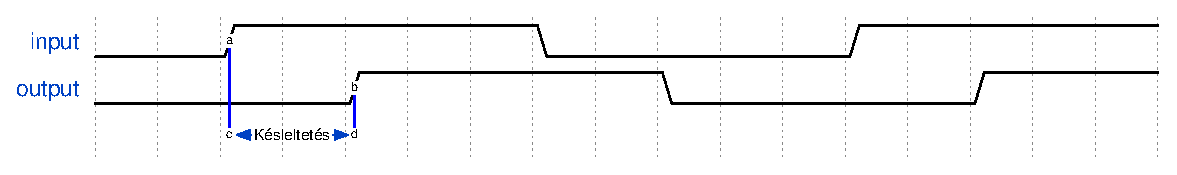
\includegraphics{figures/Benchmark/01_latency.eps}}
\caption{Az oper�ci�s rendszer k�sleltet�s�nek szeml�ltet�se.}
\label{fig:01_latency}
\end{figure}

%----------------------------------------------------------------------------
\subsection{Jitter}
%----------------------------------------------------------------------------

A jitter egy folyamat vizsg�lata sor�n a t�bbsz�ri bek�vetkez�s ut�n m�rt k�sleltet�sekb�l hat�rozhat� meg.

\begin{figure}[h!]
\center
\resizebox{15cm}{!}{
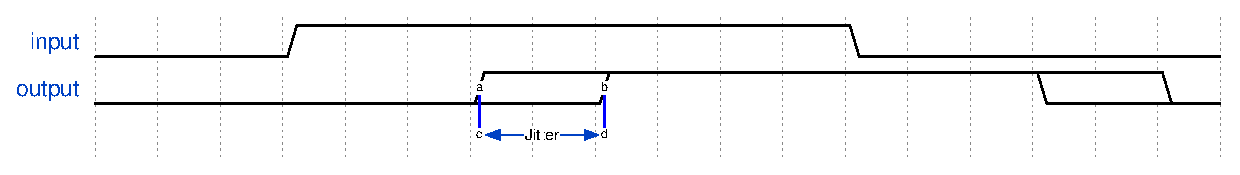
\includegraphics{figures/Benchmark/02_jitter.eps}}
\caption{A k�sleltet�s jitter�nek szeml�ltet�se.}
\label{fig:02_jitter}
\end{figure}

%----------------------------------------------------------------------------
\subsection{Rhealstone}
%----------------------------------------------------------------------------

1989-ben a Dr. Dobbs Journal cikkek�nt jelent meg egy javaslat, ami a val�sidej� rendszerek objekt�v �rt�kel�s�t c�lozta meg. Rabindra P. Kar, az Intel Systems Group senior m�rn�ke ismertette a m�dszer el�nyeit �s szempontjait, melynek a Rhealstone nevet adta\footnote{A n�v a Whetstone �s Dhrystone m�dszerek elnevez�seit k�vetve, mint sz�j�t�k ered.}.

A cikk megjelen�sekor m�r l�teztek teljes�tm�nym�r� met�dusok (p�ld�ul Whetstone, Dhrystone), de ezek a ford�t� �ltal gener�lt k�dot, illetve a hardvert min�s�tett�k. A Rhealstone metrika c�lja, hogy a fejleszt�ket seg�tse az alkalmaz�sukhoz legink�bb megfelel� oper�ci�s rendszer kiv�laszt�s�ban.

A Rhealstone hat kateg�ri�ban vizsg�lja meg az oper�ci�s rendszer k�pess�geit:
\begin{itemize}
\item Taszkv�lt�si id� (Task switching time),
\item Preempt�l�si id� (Preemption time),
\item Megszak�t�s-k�sleltet�si id� (Interrupt latency time),
\item Szemafor-v�lt�si id� (Semaphore shuffling time),
\item Deadlock-felold�si id�\footnote{A vizsg�lat sor�n nem alakul ki t�nyleges holtpont. A m�r�s a priorit�s-inverzi� jelens�g�t szimul�lja, de az eredeti forr�s tisztelet�re megtartottam a terminol�gi�t.} (Deadlock breaking time),
\item Datagram-�tviteli id�\footnote{B�r a kateg�ria neve id�nek nevezi a m�rt mennyis�get, az eredeti dokumentum alapj�n a m�r�s $\sfrac{kB}{sec}$-ben �rtelmezett adatot eredm�nyez. Ha az 1~kB �tvitel�hez sz�ks�ges id�t m�rj�k, akkor viszont megold�dik ez a probl�ma.} (Datagram throughput time).
\end{itemize}

1990-ben megjelent egy m�sodik cikk is, amelyben amellett, hogy az egyes kateg�ri�k p�ldaprogramjait k�z�lt�k (iRMX oper�ci�s rendszerhez), p�r kateg�ria meghat�roz�s�t megv�ltoztatt�k. Ezen v�ltoztat�sokat az adott kateg�ria r�szletez�sekor ismertetem.

%----------------------------------------------------------------------------
\subsubsection{Taszkv�lt�si id�}
%----------------------------------------------------------------------------

A taszkv�lt�si id� a k�t f�ggetlen, fut�sra k�sz, azonos priorit�s� taszkok v�lt�s�hoz sz�ks�ges �tlagos id�tartam.

\begin{figure}[h!]
\center
\resizebox{13cm}{!}{
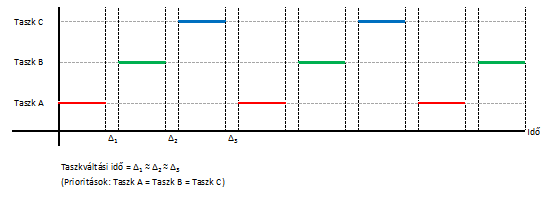
\includegraphics{figures/Benchmark/03_task_switching_time.png}}
\caption{A taszv�lt�si id� szeml�ltet�se.}
\label{fig:03_task_switching_time}
\end{figure}

A taszkv�lt�si id� alapvet� jellemz�je egy multitaszk rendszernek. A m�r�s a taszkokat nyilv�ntart� strukt�r�k hat�konys�g�r�l ad k�pet. A taszkv�lt�si id�t a haszn�lt processzor architekt�r�ja, utas�t�sk�szlete is befoly�solja.

A rendszerek a futtathat� taszkokat �ltal�ban valamilyen list�ban t�rolj�k, �gy k�l�nb�z� sz�m� taszkkal elv�gezve a m�r�st m�s eredm�nyt kaphatunk.

%----------------------------------------------------------------------------
\subsubsection{Preempt�l�si id�}
%----------------------------------------------------------------------------

A preempt�l�si id� egy magasabb priorit�s� taszk �rv�nyre jut�s�hoz sz�ks�ges �tlagos id�tartam.

\begin{figure}[h!]
\center
\resizebox{13cm}{!}{
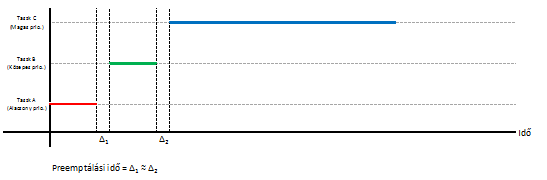
\includegraphics{figures/Benchmark/04_preemption_time.png}}
\caption{A preempt�l�si id� szeml�ltet�se.}
\label{fig:04_preemption_time}
\end{figure}

A preempt�l�si id� nagyban hasonl�t a taszkv�lt�si id�h�z, azonban a j�rul�kos utas�t�sok miatt �ltal�ban hosszabb id�t jelent.

%----------------------------------------------------------------------------
\subsubsection{Megszak�t�s-k�sleltet�si id�}
%----------------------------------------------------------------------------

A megszak�t�s-k�sleltet�si id� egy esem�ny be�rkez�se �s a megszak�t�s-kezel� rutin els� utas�t�sa k�z�tt eltelt �tlagos id�tartam.

\begin{figure}[h!]
\center
\resizebox{13cm}{!}{
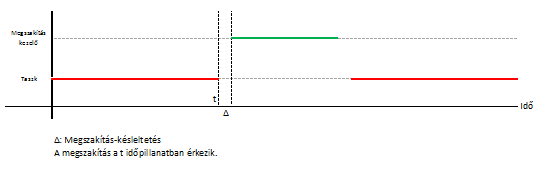
\includegraphics{figures/Benchmark/05_interrupt_latency_time.png}}
\caption{A megszak�t�s-k�sleltet�si id� szeml�ltet�se.}
\label{fig:05_interrupt_latency_time}
\end{figure}

%----------------------------------------------------------------------------
\subsubsection{Szemafor-v�lt�si id�}
%----------------------------------------------------------------------------

Az 1989-es cikk szerint szemafor-v�lt�si id� az az �tlagos id�tartam, ami egy szemafor elenged�se �s egy, a szemaforra v�rakoz� taszk elindul�sa k�z�tt eltelik (\figref{06_semaphore_shuffling_time_1}a).

\begin{figure}[h!]
\center
\resizebox{13cm}{!}{
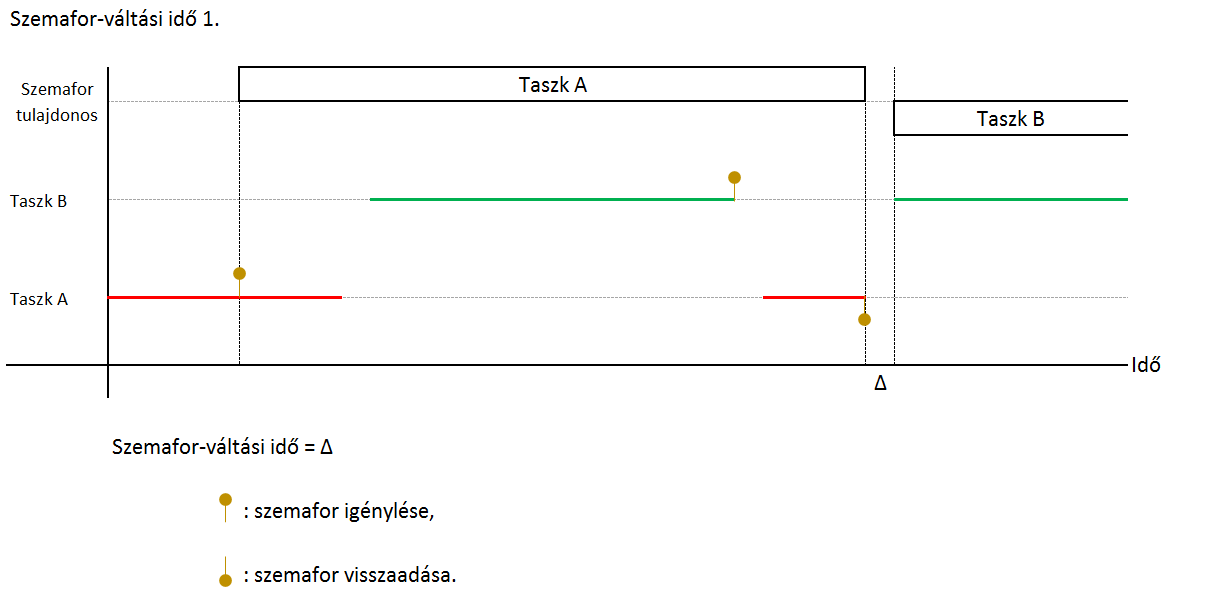
\includegraphics{figures/Benchmark/06_semaphore_shuffling_time_1.png}}
\caption{A szemafor-v�lt�si id� szeml�ltet�se (1989-es meghat�roz�s alapj�n).}
\label{fig:06_semaphore_shuffling_time_1}
\end{figure}

Ezt a meghat�roz�st 1990-ben annyival m�dos�tott�k, hogy a szemafor-v�lt�si id� egy m�r birtokolt szemafor k�r�se �s a k�r�s teljes�t�se k�z�tt eltelt id�tartam, a birtokl� taszk fut�si idej�t�l eltekintve (\figref{07_semaphore_shuffling_time_2}a).

\begin{figure}[h!]
\center
\resizebox{13cm}{!}{
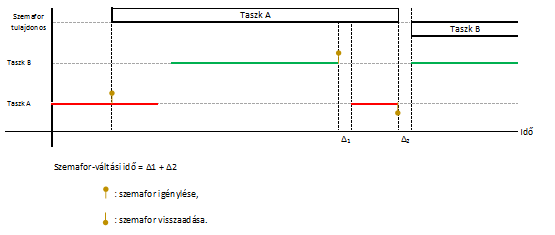
\includegraphics{figures/Benchmark/07_semaphore_shuffling_time_2.png}}
\caption{A szemafor-v�lt�si id� szeml�ltet�se (1990-es meghat�roz�s alapj�n).}
\label{fig:07_semaphore_shuffling_time_2}
\end{figure}

A m�r�s c�lja az overhead meghat�roz�sa, mikor egy szemafor k�lcs�n�s kiz�r�st (mutex) val�s�t meg.

%----------------------------------------------------------------------------
\subsubsection{Deadlock-felold�si id�}
%----------------------------------------------------------------------------

A deadlock-felold�si id� az az �tlagos id�tartam, ami egy olyan er�forr�s el�r�s�hez sz�ks�ges, amit egy alacsonyabb priorit�s� taszk m�r birtokol (\figref{08_deadlock_breaking_time}a).

\begin{figure}[h!]
\center
\resizebox{13cm}{!}{
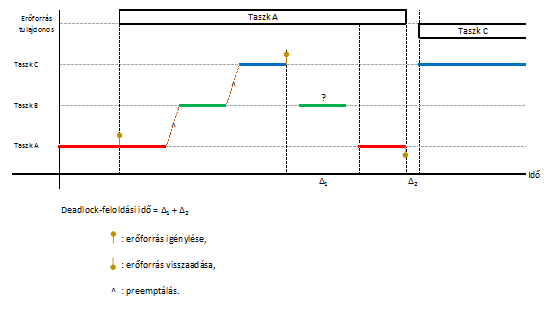
\includegraphics{figures/Benchmark/08_deadlock_breaking_time.png}}
\caption{A deadlock-felold�si id� szeml�ltet�se.}
\label{fig:08_deadlock_breaking_time}
\end{figure}

Vagyis a deadlock-felold�si id� a birtokl�si probl�ma felold�s�hoz sz�ks�ges �sszes�tett id� egy alacsony �s egy magas priorit�s� taszk k�z�tt.

%----------------------------------------------------------------------------
\subsubsection{Datagram-�tviteli id�}
%----------------------------------------------------------------------------

A datagram-�tviteli id� a taszkok k�z�tt el�rhet� adatsebess�g az oper�ci�s rendszer objektumait kihaszn�lva (vagyis nem megosztott mem�ri�n vagy pointeren kereszt�l). Az adatk�ld� taszknak kapnia kell �rtes�t�st az adat �tv�tel�r�l (\figref{09_datagram_throughput_time}a).

\begin{figure}[h!]
\center
\resizebox{13cm}{!}{
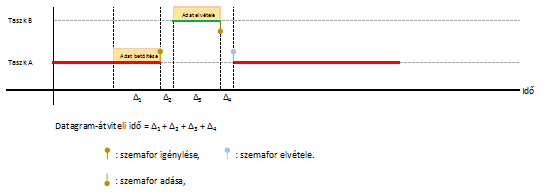
\includegraphics{figures/Benchmark/09_datagram_throughput_time.png}}
\caption{A datagram-�tviteli id� szeml�ltet�se.}
\label{fig:09_datagram_throughput_time}
\end{figure}

Az egy �vvel k�s�bb megjelent cikkben ezt a kateg�ri�t is m�dos�tott�k kis m�rt�kben. Egyr�szt a megnevez�st taszk k�z�tti �zenet-k�sleltet�sre v�ltoztatt�k, m�sr�szt nem a maxim�lis adatsebess�g meghat�roz�sa a m�r�s c�lja, hanem az adattov�bb�t�st v�gz� objektum kezel�s�nek �s az oper�ci�s rendszer j�rul�kos m�veleteinek hat�konys�g�nak megm�r�se (\figref{10_intertask_message_latency}a).

\begin{figure}[h!]
\center
\resizebox{13cm}{!}{
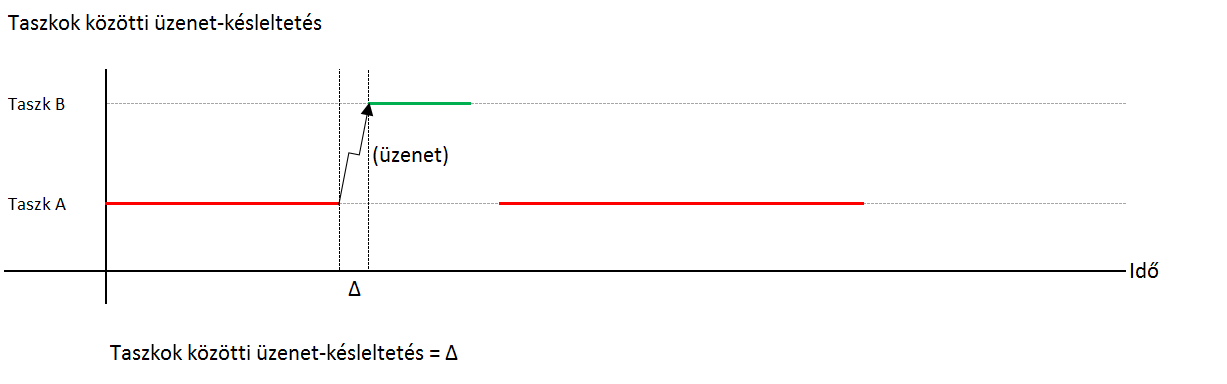
\includegraphics{figures/Benchmark/10_intertask_message_latency.png}}
\caption{A taszk k�z�tti �zenet-k�sleltet�si id� szeml�ltet�se.}
\label{fig:10_intertask_message_latency}
\end{figure}

%----------------------------------------------------------------------------
\subsubsection{Rhealstone jellemz�k �sszegz�se}
%----------------------------------------------------------------------------

Az elv�gzett m�r�sek v�rhat�an mikroszekundum �s milliszekumdum nagys�grend� �rt�keket adnak vissza. Minden �rt�ket m�sodpercre v�ltva, majd a reciprok�t v�ve az �rt�kek �sszegezhet�ek egy reprezentat�v �rt�kk�. Az �tv�lt�snak k�sz�nhet�en a nagyobb �rt�k jobb teljes�tm�nyt jelent, ami a teljes�tm�nymutat�k vil�g�ban elv�rt.

%----------------------------------------------------------------------------
\paragraph{Objekt�v Rhealstone �rt�k}
%----------------------------------------------------------------------------

Objekt�v �rt�kel�s eset�n minden jellemz� azonos s�llyal szerepel a sz�mol�s sor�n (\eqref{objective_rhealstone}~k�plet).

\begin{align}
\label{eq:objective_rhealstone}
& r_{1}+r_{2}+r_{3}+r_{4}+r_{5}+r_{6}=\sfrac{\textrm{objekt�v Rhealstone}}{\textrm{sec}},\\[5pt]
& \textrm{ahol} \nonumber \\
& \qquad r_{1}\textrm{ a taszkv�lt�si id�b�l sz�rmaz� �rt�k,} \nonumber \\
& \qquad r_{2}\textrm{ a preempt�l�si id�b�l sz�rmaz� �rt�k,} \nonumber \\
& \qquad \textrm{�s �gy tov�bb}. \nonumber
\end{align}

%----------------------------------------------------------------------------
\paragraph{S�lyozott Rhealstone �rt�k}
%----------------------------------------------------------------------------

Az esetek d�nt� t�bbs�g�ben a vizsg�lt feladatok nem azonos gyakoris�ggal szerepelnek egy alkalmaz�sban, s�t, el�fordulhat, hogy valamely funkci�t nem is haszn�l az alkalmaz�s. Ekkor informat�vabb eredm�nyt kapunk, ha az egyes jellemz�kre kapott sz�m�rt�keket k�l�nb�z� s�llyal vessz�k bele a v�geredm�ny meghat�roz�s�ba (\eqref{application_rhealstone}~k�plet).

\begin{align}
\label{eq:application_rhealstone}
& n_{1}\cdot r_{1}+n_{2}\cdot r_{2}+n_{3}\cdot r_{3}+n_{4}\cdot r_{4}+n_{5}\cdot r_{5}+n_{6}\cdot r_{6}=\\
&\mkern360mu\sfrac{\textrm{alkalmaz�s specifikus Rhealstone}}{\textrm{sec}}, \nonumber \\[5pt]
& \textrm{ahol} \nonumber \\
& \qquad n_{1}\textrm{ a taszkv�lt�si id�h�z tartoz� s�lyt�nyez�,} \nonumber \\
& \qquad r_{1}\textrm{ a taszkv�lt�si id�b�l sz�rmaz� �rt�k,} \nonumber \\
& \qquad n_{2}\textrm{ a preempt�l�si id�h�z tartoz� s�lyt�nyez�,} \nonumber \\
& \qquad r_{2}\textrm{ a preempt�l�si id�b�l sz�rmaz� �rt�k,} \nonumber \\
& \qquad \textrm{�s �gy tov�bb}. \nonumber
\end{align}

Az s�lyt�nyez�k �rt�ke nulla is lehet.

%----------------------------------------------------------------------------
\subsection{Legrosszabb v�laszid�}
%----------------------------------------------------------------------------

2001-ben a Nemzetk�zi Automatiz�l�si T�rsas�g (International Society of Automation - ISA) egy jelent�sben fejtette ki azt az �ll�spontj�t, miszerint a k�sleltet�s nem jellemzi a val�sidej� rendszert, mert lehet, hogy a legt�bb esetben az el��rt id�n bel�l v�laszol, de ritk�n el�fordulhatnak k�sleltet�sek vagy kihagyott esem�nyek, amiket a m�r�s sor�n nem lehet detekt�lni.

A T�rsas�g egy olyan m�r�si �ssze�ll�t�st javasol a fejleszt�knek, ami egyszer�s�ge ellen�re k�pes meghat�rozni a rendszer legrosszabb v�laszidej�t (\figref{11_worst_case_response_time}a).

A m�r�shez sz�ks�ges eszk�z�k:
\begin{itemize}
\item M�rend� rendszer (legal�bb egy be- �s kimenettel),
\item Jelgener�tor.
\item K�t darab digit�lis sz�ml�l�.
\end{itemize}

%----------------------------------------------------------------------------
\subsubsection{M�r�si elrendez�s}
%----------------------------------------------------------------------------

A jelgener�tor kimenet�t a m�rend� rendszer bemenet�re, illetve mindk�t sz�ml�l� \emph{count up} bemenet�re k�tj�k, m�g a m�rend� rendszer kimenet�t a kimeneti sz�ml�l� \emph{count down} bemenet�re k�tj�k.

\begin{figure}[h!]
\center
\resizebox{13cm}{!}{
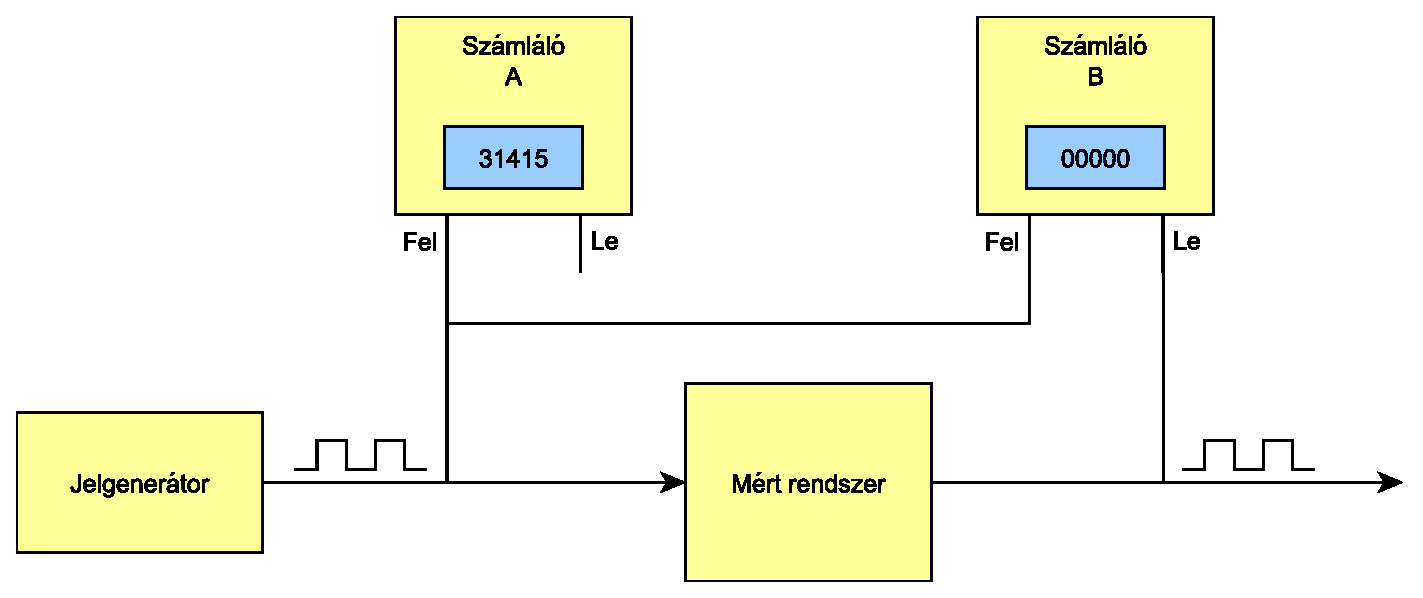
\includegraphics{figures/Benchmark/11_worst_case_response_time.eps}}
\caption{A legrosszabb v�laszid� m�r�si �ssze�ll�t�sa.}
\label{fig:11_worst_case_response_time}
\end{figure}

%----------------------------------------------------------------------------
\subsubsection{M�r�si elv}
%----------------------------------------------------------------------------

A m�r�s sor�n azt a legkisebb frekvenci�t keress�k, amit a rendszer m�r nem tud k�vetni, vagyis impulzusokat vesz�t. Ez�ltal a kimenet�n megjelen� impulzusok sz�ma k�l�nb�zni fog a bemenet�re adott impulzusok sz�m�t�l, amit a sz�ml�l�k seg�ts�g�vel detekt�lunk. A kapott frekvencia a legrosszabb v�laszid� reciproka.

%----------------------------------------------------------------------------
\subsubsection{M�r�s menete}
%----------------------------------------------------------------------------

\begin{enumerate}
\item A rendszeren fut� program a bemenet�re �rkez� jelet a kimenet�re m�solja. A m�r�s sor�n digit�lis �s anal�g I/O l�b is haszn�lhat�.
\item M�r�si eszk�z�k csatlakoztat�sa.
\item Alacsony frekvenci�r�l indulva n�velj�k a bemeneti jel frekvenci�j�t. Az \emph{A} sz�ml�l� folyamatosan sz�mol felfele. Am�g a rendszer k�pes k�vetni a bemenetet, addig a \emph{B} sz�ml�l� 1 �s 0 k�z�tt v�ltakozik. Amikor a rendszer m�r nem k�pes k�vetni a bemenetet, akkor a \emph{B} sz�ml�l� elkezdt felfele sz�molni.
\item Cs�kkentj�k a bemeneti frekvencia �rt�k�t eg�szen addig, am�g a rendszer �jb�l k�pess� nem v�lik a bemenet k�vet�s�re. A kapott frekvencia a legrosszabb v�laszid� reciproka.
\end{enumerate}

A m�r�st c�lszer� elv�gezni k�l�nb�z� terhel�s mellett. Ha valamelyik funkci� haszn�lata k�zben (adatt�rol� vez�rl�se, h�l�zati kommunik�ci�, stb.) a \emph{B} sz�ml�l� elindul, akkor az adott frekvenci�n a rendszer nem determinisztikus.

%----------------------------------------------------------------------------
\section{Vizsg�lt oper�ci�s rendszer jellemz�k}
%----------------------------------------------------------------------------

A feladat megold�sa sor�n els�dlegesen az oper�ci�s rendszerek jellemz�it vizsg�lom, ez�rt nem ker�lnek k�l�n tesztel�sre az egyes hardverek el�nyei. Az egyes rendszer-jellemz�ket terheletlen�l �s terhel�s alatt is megm�rem.

Egy ipari alkalmaz�s szimul�ci�j�t is megval�s�tom, mely egy m�sik �sszehasonl�t�si alapot ny�jt a dolgozathoz. Az alkalmaz�st felhaszn�lom a terhel�s alatti m�r�s megval�s�t�s�hoz is.

A dolgozat tov�bbi r�szeiben \asecref{metrics}ben felsorolt �sszes jellemz� meghat�roz�s�ra k�pes rendszert �ll�tok �ssze, mellyel v�grehajtom a m�r�seket. A meghat�rozand� jellemz�k:
\begin{itemize}
\item Mem�riaig�ny,
\item K�sleltet�s,
\item Jitter,
\item Rhealstone �rt�kek (els� publik�ci� szerinti �rt�kek),
\item Legrosszabb v�laszid�.
\end{itemize} 
%----------------------------------------------------------------------------
\chapter{Rendszerterv}
%----------------------------------------------------------------------------

%----------------------------------------------------------------------------
\section{Megval�s�tand� feladat}
%----------------------------------------------------------------------------

%----------------------------------------------------------------------------
\section{Kapcsol�si rajz}
%----------------------------------------------------------------------------

%----------------------------------------------------------------------------
\section{Nyomtatott �ramk�ri terv}
%----------------------------------------------------------------------------

%----------------------------------------------------------------------------
\section{Szoftverterv}
%----------------------------------------------------------------------------
%----------------------------------------------------------------------------
\chapter{Megval�s�t�s}
%----------------------------------------------------------------------------

%----------------------------------------------------------------------------
\section{STM32F4~Discovery}
%----------------------------------------------------------------------------

A STM32F4~Discovery k�rty�ra val� fejleszt�s sor�n az \emph{Atollic~TrueSTUDIO} fejleszt�k�rnyezet ingyenes verzi�j�t, illetve az \emph{STM32CubeMX} konfigur�l� alkalmaz�st haszn�ltam. Mindk�t oper�ci�s rendszern�l kikapcsoltam az optimaliz�ci�t.

%----------------------------------------------------------------------------
\subsection{FreeRTOS}
\label{sec:freertosImplementation}
%----------------------------------------------------------------------------

Az STM honlapj�r�l let�lthet� STM32CubeMX alkalmaz�s t�mogatja a FreeRTOS �s FatFS\footnote{Fat f�jlrendszer haszn�lat�hoz el�rhet� k�nyvt�r, mely az SD k�rtya haszn�lat�hoz sz�ks�ges.} haszn�lat�t, �gy a megfelel� perif�ri�k be�ll�t�sa �s a sz�ks�ges modulok kiv�laszt�sa ut�n m�k�d� p�ldaprogram gener�lhat�.

A gener�lt k�d �ttekint�se k�zben �szrevettem, hogy az oper�ci�s rendszer f�ggv�nyeinek nevei nem egyeznek meg \asecref{freertos}ben megismert f�ggv�nyek neveivel. Ennek oka, hogy a CubeMX a FreeRTOS f�ggv�nyeit a CMSIS-RTOS API-val elfedi, �s egy egyszer�s�tett fel�letet biztos�t a fejleszt� sz�m�ra. Ez az egyszer�s�tett fel�let p�ld�ul a szemaforok haszn�lat�n�l figyelhet� meg, ahol nincs k�l�n met�dus a megszak�t�sb�l t�rt�n� haszn�latra, hanem az API vizsg�lja meg, hogy megszak�t�s-kezel� rutinb�l t�rt�nt-e a h�v�s, �s ennek megfelel�en v�gzi el a tov�bbi m�veleteket. Mivel az �sszehasonl�t�s sor�n a fejleszt�si folyamat neh�zs�gei is szempontk�nt szerepelnek, ez�rt �ltem az API haszn�lat�val.

Miel�tt \asecref{softwareDesign}ben ismertetett taszkokat implement�ltam volna, a rendszer megismer�s�vel foglalkoztam. Valahogy el kellett �rnem, hogy az �ppen fut� taszkhoz azonos�t�t rendeljek, amit valahogy az ID l�bakon jelezni is tudok. Ehhez kihaszn�ltam azt, hogy minden taszk rendelkezik n�vvel, �gy megfontolt elnevez�ssel minden taszkhoz rendelhet� 4~bites azonos�t�, amit a TCB-b�l is egyszer�en kiolvashatok.

Az ASCII karakterek t�bl�zat�t megvizsg�lva l�that�, hogy az ``A'' karaktert�l kezd�d�en a bet�k als� bitjei haszn�lhat�ak az ID l�bak �rt�k�nek meghat�roz�s�ra. Az azonos�t�k kioszt�s�n�l �gy d�nt�ttem, hogy a $0\textrm{x}0$ �rt�k tartozzon az �temez�h�z, a $0\textrm{x}1$ az Idle taszkhoz, �s a nagyobb �rt�kek tartozzanak a m�r�sben r�szt vev� taszkokhoz. �gy az egyes taszkok nevei ``B''-t�l ``O''-ig terjedhetnek.

A k�vetkez� l�p�s volt a rendszer �temez�si mechanizmus�nak tanulm�nyoz�sa. Meg kellett keresnem azokat a r�szeket, amelyek minden �temez�sn�l lefutnak, �s az �temez�s indul�sakor a $0\textrm{x}0$ azonos�t�t kellett kitennem az ID l�bakra, m�g az �temez�s v�g�n a kiv�lasztott taszk azonos�t�j�t. A FreeRTOS k�t esetben futtatja le az �temez�t:
\begin{itemize}
  \item SysTick esem�ny bek�vetkez�sekor,
  \item portYIELD() f�ggv�ny h�v�sakor.
\end{itemize}

Ez�rt a \emph{portYIELD()} f�ggv�ny elej�n, illetve a \emph{SysTick} megszak�t�s-kezel� rutin elej�n \alstref{schedulerID}�ban l�that� assembly utas�t�sokkal helyeztem ki az �temez� azonos�t�j�t. A \emph{portYIELD()} f�ggv�ny minden esetben kontextus-v�lt�st k�r a \emph{PendSV} megszak�t�son kereszt�l, ellenben a \emph{SysTick} kezel� csak sz�ks�ges esetben. Emiatt a \emph{SysTick} rutint m�dos�tanom kellett, �s amennyiben nem sz�ks�ges kontextus-v�lt�s, �gy az aktu�lis taszk azonos�t�j�t helyezem az ID l�bakra.

Kontextus-v�lt�s eset�n a \emph{PendSV} megszak�t�s-kezel� v�gzi el az �ppen fut� taszk �llapot�nak elment�s�t �s a soron k�vetkez� taszk legutols� �llapot�nak bet�lt�s�t. A taszkv�lt�s elv�gz�se ut�n, a megszak�t�sb�l val� visszat�r�s el�tt a bet�lt�tt taszk azonos�t�j�t helyezem az ID l�bakra \alstref{freertosTaskID}�ban l�that� m�don.

A taszk nev�nek el�r�s�hez a FreeRTOS-ban haszn�lt TCB strukt�ra v�ltoz�t kellett lesz�molnom. A taszk neve el�tti v�ltoz�k �sszesen $52$~byte hossz�ak, ebb�l ad�dik \alstref{freertosTaskID}a hatodik sor�ban tal�lhat� konstans ofszet.

\begin{lstlisting}[caption={�temez� azonos�t�j�nak kihelyez�se a l�bakra.}\label{lst:schedulerID},numbers={left}]
"   push {r0, r1, r2}             \n"
"   movw r0, #0x0C14              \n" /* GPIOD cimenek betoltese */
"   movt r0, #0x4002              \n"
"   ldr r2,[r0, #0]               \n"
"   and r2, r2, #0xFFFFFF0F       \n"
"   str r2, [r0, #0]              \n" /* Null ertekek kiirasa a labakra */
"   pop {r0, r1, r2}              \n"		
\end{lstlisting}

\begin{lstlisting}[caption={Aktu�lis taszk azonos�t�j�nak kihelyez�se a l�bakra (FreeRTOS).}\label{lst:freertosTaskID},numbers={left}]
"   push {r0, r1, r2}             \n"
"   ldr	r0, pxCurrentTCBConst     \n" /* Aktualis TCB betoltese. */
"   ldr	r2, [r0]                  \n"
"   movw r0, #0x0C14              \n" /* GPIOD cimenek betoltese */
"   movt r0, #0x4002              \n"
"   ldr r1, [r2, #52]             \n" /* Taszk ID kiolvasas */
"   lsl r1, r1, #4                \n" /* ID helyre mozgatasa */
"   and r1, r1, #0x000000F0       \n" /* Maszkolasok */
"   ldr r2, [r0, #0]              \n"
"   and r2, r2, #0xFFFFFF0F       \n"
"   orr r2, r2, r1                \n"
"   str r2, [r0, #0]              \n" /* Ertek kihelyezese a labakra */
"   pop {r0, r1, r2}              \n"
\end{lstlisting}

A m�dos�t�sok tesztel�se ut�n \asecref{softwareDesign}ben bemutatott taszkok implement�l�sa k�vetkezett.

Minden m�r�snek �j projektet l�trehozni nem lett volna c�lszer�, ez�rt makr�k seg�ts�g�vel lehet kiv�lasztani az aktu�lis m�r�st. A konfigur�ci�s f�jl r�szlete l�that� \alstref{measurementDefines}�n\footnote{A \emph{BLINKING\_LED} a fejleszt�s sor�n seg�tette a hib�s m�k�d�s �szrev�tel�t.}.

A k�vetkez� l�p�s az ipari alkalmaz�s implement�ci�ja volt. Minden taszk m�k�d�s�nek ismertet�se hosszadalmas -- �s egyben felesleges is -- volna, ez�rt csak a fejleszt�s szempontj�b�l �rdekes r�szleteket emelem ki.

A t�voli fel�gyeletet soros kommunik�ci� seg�ts�g�vel val�s�tottam meg, amihez c�lszer� volt valamilyen egyszer� protokollt meghat�roznom. Mivel t�bb szenzor adat�t is tov�bb�tanom kellett, �s a k�ld�tt inform�ci�k sorrendje v�ltozhatott, ez�rt a protokollnak tartalmaznia kellett az adatok forr�s�t. A legnagyobb tov�bb�tand� �rt�k $4$~byte hossz� volt, ez�rt az �zenet form�tum�t az al�bbi m�don hat�roztam meg:
\begin{itemize}
  \item Az adat forr�sa (szenzor neve) nyolc karakteren,
  \item Elv�laszt� karakter (:),
  \item Adat ($4$~byte),
  \item Lez�r� karakter (sort�r�s).
\end{itemize}

\begin{lstlisting}[language=C,numbers={left},keywordstyle={\color{blue}},stringstyle={\color{red}},commentstyle={\color{olive}},morecomment={[l][\color{red}]{\#}},tabsize=2, caption={M�r�s kiv�laszt�s�t megval�s�t� makr�k.} \label{lst:measurementDefines}]
/**
 * M�r�si folyamat:
 *  MEAS_LATENCY:                   k�sleltet�s m�r�s
 * 	MEAS_TASK_SWITCHING_TIME:       taszkv�lt�si id� m�r�s
 * 	MEAS_PREEMPTION_TIME:           preemt�l�si id� m�r�s
 * 	MEAS_INTERRUPT_LATENCY_TIME:    megszak�t�s-k�sleltet�si id� m�r�s
 * 	MEAS_SEMAPHORE_SHUFFLING_TIME:  szemafor-v�lt�si id� m�r�s
 * 	MEAS_DEADLOCK_BREAKING_TIME:    deadlock-felold�si id� m�r�s
 * 	MEAS_DATAGRAM_THROUGHPUT_TIME:  datagram-�tviteli id� m�r�s
 */
/**
 * Terhel�s enged�lyez�se:
 *  MEAS_W_LOAD
 */
#define MEAS_LATENCY
//#define BLINKING_LED
//#define MEAS_W_LOAD
\end{lstlisting}

A kommunik�ci� sor�n el�fordul, hogy a mikrokontroller sz�m�ra k�ld�tt karakter nem ker�l id�ben fogad�sra, �s a perif�ria t�rol�ja t�lcsordul. Ekkor a perif�ria kezel�se ut�n az alkalmaz�s jelez a t�voli vez�rl�nek, hogy k�ldje �jra az utols� parancsot.

Az SD k�rty�ra val� napl�z�s sor�n k�t probl�ma mer�lt fel, melynek megold�sa hosszabb id�t vett ig�nybe. Egyr�szt amikor a napl�f�jl m�rete el�rte a k�rtya form�z�sa sor�n megadott szektorm�retet, akkor az �r�s nem folytat�dott. Erre hosszas kutat�s ut�n sem tal�ltam elfogadhat� megold�st, viszont a f�jl m�dos�t�s�t v�gz� f�ggv�nyek kritikusz szakaszba �gyaz�s�val a probl�ma megold�dott\footnote{Mivel a f�jl kezel�se viszonylag hossz� ideig tart, ez�rt ez a megold�s egy val�s alkalmaz�sban nem felelne meg!}. A m�sik probl�ma akkor jelentkezett, ha m�k�d�s k�zben elt�vol�tottam a mem�ria k�rty�t, majd �jb�l visszahelyeztem a foglalatba. A visszahelyez�s ut�n a k�rty�ra val� �r�s nem t�rt�nt meg, a kezel� f�ggv�nyek hib�val t�rtek vissza. A \emph{FatFS} f�gv�nyeinek tanulm�nyoz�s�val azt vettem �szre, hogy tagv�ltoz�ban t�rolja, hogy az adott eszk�z inicializ�l�sa megt�rt�nt-e. Az inicilaiz�l�st t�rol� v�ltoz�t csak az eszk�zt kezel� \emph{driver} be�ll�t�sakor t�rli, �gy a k�rtya inicializ�l�sa a t�bbsz�ri behelyez�s eset�n nem val�sul meg. Az alkalmaz�sban a k�rtya lecsatol�sakor t�rl�m a v�ltoz� �rt�k�t.

A BLE112 Bluetooth modul kezel�s�hez sz�ks�ges f�ggv�nyek k�nyvt�r�t a gy�rt� a fejleszt�k sz�m�ra regisztr�ci� ut�n el�rhet�v� teszi. A fejleszt�nek csak az adatok k�ld�s�t �s fogad�s�t megval�s�t� f�ggv�nyeket kell implement�lnia. A fogad� f�ggv�ny a bej�v� adatot feldolgozza, majd megh�vja az �zenethez tartoz� f�ggv�nyt, ahol a sz�ks�ges feladatokat elv�gezhetj�k.

A soros kommunik�ci� �s a napl�z�s sor�n \emph{gatekeeper} taszkokkal val�s�tottam meg az er�forr�sok kezel�s�t.

Az egyes taszkok m�k�d�se \aappref{flowCharts}ben tal�lhat�.

%----------------------------------------------------------------------------
\subsection{\textmugreek C/OS--III}
%----------------------------------------------------------------------------

A \textmugreek C/OS--III �temez�je szint�n a \emph{SysTick} esem�nyt haszn�lja a periodikus �temez�s megval�s�t�s�ra, viszont a mechanizmus k�l�nb�zik a FreeRTOS eset�ben megismertt�l.

A Idle taszk mellet az oper�ci�s rendszer inicializ�l�sakor l�trej�n \emph{Tick} taszk is, ami periodikusan v�rakozik a be�p�tett szemafor�ra. \emph{SysTick} megszak�t�s �rkez�sekor a megszak�t�s-kezel� rutin jelez a Tick taszknak a szemaforon kereszt�l, majd a \emph{Pend} f�ggv�nyh�v�s k�vetkezt�ben az �temez� lefut. Mivel a \emph{Tick} taszk magas priorit�ssal rendelkezik, ez�rt a k�sleltet�s kicsi. A Tick taszk elv�gzi a sz�ml�l�k kezel�s�t, majd v�rakozik a k�vetkez� jelz�sre, ezzel �jabb �temez�st elind�tva.

A taszkok �temez�s�st az \emph{OSSched()} f�ggv�ny v�gzi, amely sz�ks�g eset�n a \emph{PendSV} megszak�t�sok kereszt�l k�r kontextus v�lt�st.

A \textmugreek C/OS--III eset�ben az �temez� azonos�t�j�t az \emph{OSSched()} f�ggv�ny elej�n, illetve a \emph{SysTick} esem�ny bek�vetkez�sekor kellett kitennem az ID l�bakra (a FreeRTOS eset�ben megismert utas�t�sok seg�ts�g�vel -- \lstref{schedulerID}a).

Az \emph{OSSched()} lefut�sa sor�n k�t lehet�s�g �ll fenn:
\begin{itemize}
  \item Nem sz�ks�ges kontextusv�lt�st kezdem�nyezni. Ebben az esetben az \emph{OSSched()} f�ggv�ny visszat�r�se el�tt t�rt�nik meg az aktu�lis taszk azonos�t�j�nak kit�tele az ID l�bakra.
  \item Kontextusv�lt�s k�vetkezik be. Ekkor a \emph{PendSV} megszak�t�s befejez�d�se el�tt ker�l az azonos�t� kihelyez�sre.
\end{itemize}

A \textmugreek C/OS--III TCB strukt�r�ja k�l�nb�zik a FreeRTOS-n�l haszn�lt TCB strukt�r�j�t�l. Egyr�szt a TCB nem tartalmazza a nevet, csak arra mutat� pointert, m�sr�szt a TCB kezdet�t�l sz�m�tott ofszet is k�l�nb�zik. Az ofszet �rt�ke $32$~byte, mely \alstref{ucosTaskID}�ban az �t�dik sorban l�that�. A kinyert mem�riac�mr�l m�g be kell olvasni az azonos�t�t, ami a kilencedik sorban t�rt�nik.

A \textmugreek C/OS--III a szemaforok �s sorok mellett t�mogatja a k�zvetlen�l a taszkoknak k�ld�tt jelz�sek �s �zenetek haszn�lat�t, mely hat�konyabb fut�s eredm�nyez. Mivel a k�t rendszer �sszehasonl�t�sa volt a c�l, ez�rt �gy d�nt�ttem, hogy azonos implement�ci�t haszn�lok, �s nem haszn�lom a be�p�tett objektumokat.

Az datagram-�tviteli id� taszkjainak implement�ci�ja sor�n felmer�lt a probl�ma, hogy a \textmugreek C/OS--III az �zenetre mutat� pointereket haszn�lja a tov�bb�t�s sor�n. A m�r�s le�r�s�ban hangs�lyozva szerepelt, hogy az �tvitel ne pointer haszn�lat�val t�rt�njen, ez�rt a m�r�s sor�n a sorba az adat c�me helyett mag�t az adatot helyeztem, �s a fogad� taszk eset�ben is figyeltem, hogy helyesen olvassam ki az �zenet tartalm�t\footnote{Mivel az adattov�bb�t�s sor�n $32$~bites adatot haszn�ltam, �s az architekt�ra �ltal haszn�lt pointerek is $32$~bitesek, ez�rt a megval�s�t�s nem okozott probl�m�t. �sszetett strukt�ra �tvitele eset�n bonyolultabb lett volna a helyzet.}.

A tov�bbi taszkok implement�ci�ja �gy t�rt�nik, mint ahogy a FreeRTOS eset�ben l�thattuk.

\begin{lstlisting}[caption={Aktu�lis taszk azonos�t�j�nak kihelyez�se a l�bakra (\textmugreek C/OS--III).}\label{lst:ucosTaskID},numbers={left}]
"   push {r0, r1, r2}               \n"
"   movw r1, #:lower16:OSTCBCurPtr  \n"
"   movt r1, #:upper16:OSTCBCurPtr  \n"
"   ldr r2, [r1]                    \n"
"   ldr r0, [r2, #32]               \n" /* NamePtr betoltese */
"   mov r2, r0                      \n" /* Regiszter masolasa */
"   movw r0, #0x0C14                \n" /* GPIOD cimenek betoltese */
"   movt r0, #0x4002                \n"
"   ldr r1, [r2]                    \n" /* Taszk ID kiolvasas */
"   lsl r1, r1, #4                  \n" /* ID helyre mozgatasa */
"   and r1, r1, #0x000000F0         \n" /* Maszkolasok */
"   ldr r2, [r0, #0                 \n"
"   and r2, r2, #0xFFFFFF0F         \n"
"   orr r2, r2, r1                  \n"
"   str r2, [r0, #0]                \n" /* Ertek kihelyezese a labakra */
"   pop {r0, r1, r2}                \n"
\end{lstlisting}

%----------------------------------------------------------------------------
\subsection{Vez�rl� szoftver}
%----------------------------------------------------------------------------

A t�voli vez�rl�st megval�s�t� szoftvert Qt fejleszt�k�rnyezet haszn�lat�val val�s�tottam meg.

A vez�rl� �s az eszk�z k�z�tt a kommunik�ci�t UART\footnote{A soros kommunik�ci� be�ll�t�s�hoz a p�ldaprogramok k�z�tt megtal�lhat� \emph{Terminal} alkalmaz�st vettem alapul.} val�s�tja meg a \emph{Base Board}-on el�rhet� kivezet�sen kereszt�l. A csatlakoz�skor a vez�rl� jelzi az eszk�z sz�m�ra, amire az eszk�z a LED-ek �s kapcsol�k aktu�lis �llapot�val v�laszol. A kapott �rt�keknek megfelel�en az szoftver friss�ti a felhaszn�l�i fel�letet.

A fel�leten a helyi �s t�voli h�mr�s�klet mellett a potm�ter �ll�sa grafikusan is megjelen�t�sre ker�l, m�g a k�rnyezeti h�m�rs�klet �s a f�nyer�ss�g sz�m�rt�ke olvashat� le a fel�letr�l. Jobb oldalon a kapcsol�k �s LED-ek jelenlegi �llapot�ra utal� indik�torok l�that�ak. A LED-ek �rt�ke v�ltoztathat�.

Az eszk�zt�l �rkez� adatok a szenzorokb�l kinyert nyers adatok, melyeket a vez�rl� szoftver dolgoz fel. A Sensortag �ltal m�rt �rt�keket az adott szenzor adatlapj�ban meghat�rozott sz�mol�s alapj�n sz�moltam, m�g a helyi h�m�rs�klet eset�ben a h�m�r� adatlapj�ban tal�lhat� h�m�rs�klet--fesz�lts�g karakterisztika alapj�n v�geztem k�zel�t� sz�m�t�st. Minden �rt�k eset�n �tlagolt adat ker�l megjelen�t�sre.

A grafikus fel�let \aappref{gui} \figref{remoteControl}�j�n l�that�.

%----------------------------------------------------------------------------
\section{Raspberry~Pi~3}
%----------------------------------------------------------------------------

A Raspberry~Pi~3-on haszn�lt rendszerekn�l a Rhealstone �rt�kek m�r�se nem megval�s�that�\footnote{A Windows~10~IoT~Code forr�sk�dja nem el�rhet�, �s a Raspbian rendszer eset�ben is kernelm�dos�t�sokat k�ne eszk�z�lni.}, �s a h�tt�rben fut� t�bb t�z -- esetenk�nt t�bb sz�z -- egy�b folyamat mellett nem is lenne c�lszer�. Ez�rt a k�t rendszer eset�n a k�sleltet�s �s a legrosszabb v�laszid� ker�l meghat�roz�sra, illetve szubjet�v szempontok alapj�n �rt�kelem majd �ket.

Mintk�t rendszern�l k�t alkalmaz�s ker�lt implement�ci�ra:
\begin{itemize}
  \item A szimul�lt ipari alkalmaz�s,
  \item Grafikus fel�let n�lk�li alkalmaz�s, mely a bemenetre �rkez� jelet a kimenetre m�solja.
\end{itemize}

Az ipari alkalmaz�s eset�n az adatok az eszk�z�n ker�lnek megjelen�t�sre.

%----------------------------------------------------------------------------
\subsection{Windows 10 IoT Core}
%----------------------------------------------------------------------------

A Windows~10~IoT~Core rendszer telep�t�se a \emph{Windows 10 IoT Core Dashboard} szoftver haszn�lat�val t�rt�nik. A szoftver fel�let�n ki kell v�lasztanunk a haszn�lt fejleszt�eszk�zt (eset�nkben Raspberry~Pi~2~\&~3), a telep�teni k�v�nt rendszert �s a haszn�lt SD k�rty�t. Ezen fel�l megadhatjuk m�g az eszk�z nev�t �s az adminisztr�tori jelsz�t, illetve be�ll�that�, hogy mely ismert WiFi h�l�zat be�ll�t�sait szeretn�nk haszn�lni az eszk�z�n. A felhaszn�l�i felt�telek elfogad�s�t k�vet�en a szoftver let�lti az oper�ci�s rendszert �s telep�ti az SD k�rty�ra.

A rendszer indul�sa ut�n a Raspberry~Pi -- amennyiben kapcsol�dik a h�l�zatra -- megjelenik a megtal�lt eszk�z�k list�j�ban. Az eszk�z c�m�t b�ng�sz�be be�rva az eszk�z adminiszt�ci�s fel�let�re jutunk, ahol t�bbek k�z�tt kezelhetj�k a fut� folyamatokat �s monitorozhatjuk a rendszer terhel�s�t is. Miut�n a b�ng�sz�n kereszt�l bekapcsoljuk a \emph{Remote Desktop} szolg�ltat�st, a \emph{Windows IoT Remote Client} alkalmaz�ssal t�voli asztalk�nt is haszn�lhatjuk a rendszert.

A Windows 10 IoT Core lehet�v� teszi \emph{headed} �s \emph{headless} alkalmaz�sok fejleszt�s�t.
\begin{description}
  \item[Headed:] Rendelkezik grafikus fel�lettel. Egyszerre csak egy headed alkalmaz�s futhat.
  \item[Headless:] Nem rendelkezik grafikus fel�lettel. A h�tt�rben egyszerre ak�r t�bb headless alkalmaz�s is futhat.
\end{description}

A fejleszt�s sor�n \emph{Visual Studio 2017}-et haszn�ltam. Az �j projekt l�trehoz�s�n�l az \emph{Windows Universal} csoporton bel�l az �res sablonb�l indultam ki. A fejleszt�k�rnyezet kezel�fel�lete gyors fejleszt�st tesz lehet�v�, �gy az ipari alkalmaz�s felhaszn�l�i fel�let�nek �ssze�ll�t�sa nem okozott gondot\footnote{Raspberry Pi-n nem jelen�tettem meg az �rt�keket k�l�n grafikus elem haszn�lat�val.}.

A h�tt�rben zajl� folyamatok implement�ci�ja sor�n sem �tk�ztem komolyabb probl�m�ba, a legt�bb perif�ria be�p�tett oszt�lyok seg�ts�g�vel k�nnyen kezelhet� volt. Viszont a Bluetooth haszn�lata neh�zs�get okozott. Alapos kutat�s ut�n arra jutottam, hogy a Windows 10 UWP Bluetooth API m�g akt�v fejleszt�s alatt �ll, �s amennyiben a kommunik�ci� l�trehoz�sa siker�lne, val�sz�n�leg a tov�bbiakban �jabb probl�m�k mer�ln�nek fel. Ez�rt altenat�v megold�st kerestem, �s mivel a Raspberry Pi rendelkezik UART interf�sszel is, ez�rt a BLE112 modul haszn�lata mellett d�nt�ttem.

A Bluegiga egyik m�rn�k�nek GitHub oldal�n el�rhet� a Bluetooth modulhoz k�nyvt�r, mely az MIT licenc felt�telei mellett haszn�lhat�. \Asecref{freertosImplementation}ben ismeretett met�dusok megval�s�t�sa ut�n a kommunik�ci� az elv�rt m�don m�k�d�tt.

Az alkalmaz�s fel�lete \aappref{gui} \figref{windows10Gui}�j�n l�that�.

A headless alkalmaz�s p�r sorban megval�s�that� volt. Feliratkoztam a kijel�lt GPIO l�b v�ltoz�s�t jelz� esem�nyre, �s az esem�nyhez rendelt f�ggv�nyben a kimeneti l�bra m�soltam a bemenet �rt�k�t.

%----------------------------------------------------------------------------
\subsection{Raspbian}
%----------------------------------------------------------------------------

A linux disztib�ci� telep�t�s�hez a rendszer k�pf�jlj�t le kellett t�lteni a Raspberry Pi hivatalos weboldal�r�l, majd k�l�n szoftver seg�ts�g�vel kellett a f�jlokat az SD k�rty�ra m�solni.

A fejleszt�s megoldhat� lett volna asztali sz�m�t�g�pen, viszont a Raspbian lehet�s�gei ezt nem tett�k sz�ks�gess�. A rendszer csomagkezel�j�nek seg�ts�g�vel feltelep�tettem a Qt fejleszt�k�rnyezetet, �s mag�n a Raspberry Pi-n v�geztem a fejleszt�st.

Mivel a Qt nem rendelkezik kiemelt t�mogat�ssal a Raspberry Pi-vel kapcsolatban, ez�rt el�sz�r az egyes perif�ri�kat b�rtam m�k�d�sre.

Linux rendszerek eset�n a legt�bb perif�ria �llom�nyk�nt jelenik meg a f�jlrendszeren bel�l\cite{OpreLin}. Ez Raspbian eset�n is igaz maradt, �s a GPIO l�bakat a \verb;/sys/class/gpio/; el�r�si �tvonalon �rhetj�k el. Itt tal�lhat� \verb;export; f�jlba a haszn�lni k�v�nt l�b sz�m�t be�rva megjelenik a l�b kezel�s�t lehet�v� tev� f�jlokat tartalmaz� mappa. P�ld�ul az
\begin{lstlisting}
echo 4 > /sys/class/gpio/export
\end{lstlisting}
utas�t�s hat�s�ra l�trej�n a \verb;/sys/class/gpio/gpio4; mappa, amelyen bel�l az al�bbi f�jlok seg�ts�g�vel lehet a GPIO l�bat kezelni:
\begin{description}
  \item[direction:] Meghat�rozza, hogy a l�bat kimenetk�nt vagy bemenetk�nt haszn�ljuk. Lehets�ges �rt�kei: in, out.
  \item[value:] A l�b jelenlegi �rt�k�t olvashatjuk ki a f�jlon kereszt�l. Kimenet eset�n a f�jlba val� �r�ssal v�ltoztathatjuk meg a l�b �llapot�t. Lehets�ges �rt�kei: 0, 1.
  \item[edge:] A bemeneti l�b v�ltoz�sakor a \verb;value; f�jlb�l kiolvasott �rt�k megfelel a l�bon megfigyelhet� jelszintnek, viszont a f�jl metadatai nem v�ltoznak (mint p�ld�ul az utols� m�dos�t�s d�tuma). A \verb;edge; f�jl tartalm�nak megv�ltoztat�s�val el�rhet�, hogy az adott v�ltoz�s eset�n f�jlle�r�n kereszt�l detekt�lhat� legyen a v�ltoz�s. Lehets�ges �rt�kei: none, rising, falling, both.
\end{description}

A GPIO l�bak kezel�s�hez l�trehoztam egy oszt�lyt, ami n�gy tagf�ggv�nyt tartalmaz.

\begin{description}
  \item[Init(GPIOPin,GPIODirection):] A param�terk�nt �tadott l�bat konfigur�lja fel a szint�n param�terk�nt megadott ir�nyba.
  \item[Read():] Visszat�r a l�b aktu�lis �rt�k�vel.
  \item[Write(GPIOState):] A l�b �rt�k�t a param�terk�nt kapott �rt�kre m�dos�tja.
  \item[WatchEdge(Enable):] Enged�lyezi a l�bon bek�vetkez� v�ltoz�s detekt�l�s�t.
\end{description}

Az implement�ci� sor�n az ismertetett �llom�nyok seg�ts�g�vel inicializ�lom a l�bat. Olvas�s �s �r�s eset�n a l�bhoz tartoz� \verb;value; f�jl tartalm�t olvasom ki, illetve m�dos�tom. Az �ldetekt�l�s enged�lyez�sekor az \verb;edge; f�jl �r�s�val mind a felfut�, mind a lefut� �l v�ltoz�s�nak jelz�s�t enged�lyezem, �s \emph{QFileSystemWatcher} objektum haszn�lat�val figyelem a \verb;value; f�jl v�ltoz�s�t. Amennyiben a f�jlon v�ltoz�s t�rt�nik, �gy �sszehasonl�tom a l�b aktu�lis �rt�k�t a legut�bb kiolvasott �rt�kkel (val�ban t�rt�nt-e v�ltoz�s), �s az oszt�ly \emph{EdgeDetected(value)} signal-j�n kereszt�l jelz�st k�ld�k.

Tekintettel arra, hogy Windows 10 IoT Core rendszer eset�n nem a Raspberry Pi be�p�tett Bluetooth eszk�z�t haszn�ltam, �gy d�nt�ttem, hogy Raspbian eset�n is a BLE112 Bluetooth modul seg�ts�g�vel val�s�tom meg a vezet�k n�lk�li kommunik�ci�t. Ehhez sz�ks�g volt az utas�t�sok magas szint� kezel�s�t lehet�v� tev� objektumra, amely UART-on kereszt�l kezeli a modult.

A soros kommunik�ci� haszn�lat�t a Qt t�mogatja, �s mivel az asztali alkalmaz�sn�l is alkalmaztam, �gy a be�ll�t�sa nem okozott gondot. Viszont a Bluetooth modulhoz nem tal�ltam \Cpp{ } fejleszt�shez haszn�lhat� k�nyvt�rakat, ez�rt v�g�l a \Csh{ }programoz�s sor�n haszn�lt k�nyvt�r alapj�n implement�ltam a sz�ks�ges f�ggv�nyeket.

Az I$^\textrm{2}$C kommunik�ci� megval�s�t�s�hoz a \emph{wiringPi} f�ggv�nyk�nyvt�rat haszn�ltam.

Az perif�ri�kat egyes�vel tesztelve megbizonyosodtam a m�k�d�s�kr�l, majd a tesztel�s sor�n k�sz�tett programok felhaszn�l�s�val �ssze�ll�tottam a teljes alkalmaz�st. Az alkalmaz�s fel�let�r�l \aappref{gui} \figref{raspbianGui}�j�n l�thatunk k�pet.

A grafikus fel�let n�lk�li alkalmaz�s a Raspbian eset�ben is n�h�ny sorral megval�s�that� volt. 
%----------------------------------------------------------------------------
\chapter{Konkl�zi�}
%----------------------------------------------------------------------------
%----------------------------------------------------------------------------
\chapter*{K�sz�netnyilv�n�t�s}%\addcontentsline{toc}{chapter}{K�sz�netnyilv�n�t�s}
%----------------------------------------------------------------------------

Ez nem k�telez�, ak�r t�r�lhet� is. Ha a szerz� sz�ks�g�t �rzi, itt lehet k�sz�netet nyilv�n�tani azoknak, akik hozz�j�rultak munk�jukkal ahhoz, hogy a hallgat� a szakdolgozatban vagy diplomamunk�ban le�rt feladatokat sikeresen elv�gezze. A konzulensnek val� k�sz�netnyilv�n�t�s sem k�telez�, a konzulensnek hivatalosan is dolga, hogy a hallgat�t konzult�lja.

\listoffigures%\addcontentsline{toc}{chapter}{�br�k jegyz�ke}
\listoftables%\addcontentsline{toc}{chapter}{T�bl�zatok jegyz�ke}

\nocite{*} % ToDo: T�rlend�!!!
\bibliography{mybib}
%\addcontentsline{toc}{chapter}{Irodalomjegyz�k}
\bibliographystyle{plain}

%----------------------------------------------------------------------------
\renewcommand\appendixname{F�ggel�k}
\renewcommand\appendixpagename{F�ggel�kek}
\setcounter{chapter}{0}% Equivalent to "letter A"
\renewcommand{\thechapter}{\Alph{chapter}}%

\appendixpage

\begin{appendices}
%----------------------------------------------------------------------------

%----------------------------------------------------------------------------
\chapter{A r�videbb licencek eredeti sz�vegei}
%----------------------------------------------------------------------------

%----------------------------------------------------------------------------
\section{MIT License}
%----------------------------------------------------------------------------

\begin{Verbatim}[fontsize=\footnotesize]
The MIT License (MIT)
Copyright (c) <year> <copyright holders>

Permission is hereby granted, free of charge, to any person obtaining a
copy of this software and associated documentation files (the "Software"),
to deal in the Software without restriction, including without
limitation the rights to use, copy, modify, merge, publish, distribute,
sublicense, and/or sell copies of the Software, and to permit persons to
whom the Software is furnished to do so, subject to the following
conditions:

The above copyright notice and this permission notice shall be included
in all copies or substantial portions of the Software.

THE SOFTWARE IS PROVIDED "AS IS", WITHOUT WARRANTY OF ANY KIND, EXPRESS
OR IMPLIED, INCLUDING BUT NOT LIMITED TO THE WARRANTIES OF
MERCHANTABILITY, FITNESS FOR A PARTICULAR PURPOSE AND NONINFRINGEMENT.
IN NO EVENT SHALL THE AUTHORS OR COPYRIGHT HOLDERS BE LIABLE FOR ANY
CLAIM, DAMAGES OR OTHER LIABILITY, WHETHER IN AN ACTION OF CONTRACT,
TORT OR OTHERWISE, ARISING FROM, OUT OF OR IN CONNECTION WITH THE
SOFTWARE OR THE USE OR OTHER DEALINGS IN THE SOFTWARE.
\end{Verbatim}

%----------------------------------------------------------------------------
\section{BSD}
%----------------------------------------------------------------------------

%----------------------------------------------------------------------------
\subsection{4-clause BSD (eredeti)}
%----------------------------------------------------------------------------

\begin{Verbatim}[fontsize=\footnotesize]
Copyright (c) <year> <copyright holder> . All rights reserved.
Redistribution and use in source and binary forms, with or without
modification, are permitted provided that the following conditions are
met:

1. Redistributions of source code must retain the above copyright notice,
this list of conditions and the following disclaimer.

2. Redistributions in binary form must reproduce the above copyright
notice, this list of conditions and the following disclaimer in the
documentation and/or other materials provided with the distribution.

3. All advertising materials mentioning features or use of this software
must display the following acknowledgement:
This product includes software developed by the <organization>.

4. Neither the name of <copyright holder> nor the names of its
contributors may be used to endorse or promote products derived from this
software without specific prior written permission.

THIS SOFTWARE IS PROVIDED BY COPYRIGHT HOLDER "AS IS" AND ANY EXPRESS OR
IMPLIED WARRANTIES, INCLUDING, BUT NOT LIMITED TO, THE IMPLIED WARRANTIES
OF MERCHANTABILITY AND FITNESS FOR A PARTICULAR PURPOSE ARE DISCLAIMED.
IN NO EVENT SHALL <COPYRIGHT HOLDER> BE LIABLE FOR ANY DIRECT, INDIRECT,
INCIDENTAL, SPECIAL, EXEMPLARY, OR CONSEQUENTIAL DAMAGES (INCLUDING, BUT
NOT LIMITED TO, PROCUREMENT OF SUBSTITUTE GOODS OR SERVICES; LOSS OF USE,
DATA, OR PROFITS; OR BUSINESS INTERRUPTION) HOWEVER CAUSED AND ON ANY
THEORY OF LIABILITY, WHETHER IN CONTRACT, STRICT LIABILITY, OR TORT
(INCLUDING NEGLIGENCE OR OTHERWISE) ARISING IN ANY WAY OUT OF THE USE OF
THIS SOFTWARE, EVEN IF ADVISED OF THE POSSIBILITY OF SUCH DAMAGE.
\end{Verbatim}

%----------------------------------------------------------------------------
\subsection{3-clause BSD (m�dos�tott)}
%----------------------------------------------------------------------------

\begin{Verbatim}[fontsize=\footnotesize]
Copyright (c) <YEAR>, <OWNER>
All rights reserved.

Redistribution and use in source and binary forms, with or without
modification, are permitted provided that the following conditions are
met:

1. Redistributions of source code must retain the above copyright notice,
this list of conditions and the following disclaimer.

2. Redistributions in binary form must reproduce the above copyright
notice, this list of conditions and the following disclaimer in the
documentation and/or other materials provided with the distribution.

3. Neither the name of the copyright holder nor the names of its
contributors may be used to endorse or promote products derived from this
software without specific prior written permission.

THIS SOFTWARE IS PROVIDED BY THE COPYRIGHT HOLDERS AND CONTRIBUTORS "AS
IS" AND ANY EXPRESS OR IMPLIED WARRANTIES, INCLUDING, BUT NOT LIMITED TO,
THE IMPLIED WARRANTIES OF MERCHANTABILITY AND FITNESS FOR A PARTICULAR
PURPOSE ARE DISCLAIMED. IN NO EVENT SHALL THE COPYRIGHT HOLDER OR
CONTRIBUTORS BE LIABLE FOR ANY DIRECT, INDIRECT, INCIDENTAL, SPECIAL,
EXEMPLARY, OR CONSEQUENTIAL DAMAGES (INCLUDING, BUT NOT LIMITED TO,
PROCUREMENT OF SUBSTITUTE GOODS OR SERVICES; LOSS OF USE, DATA, OR
PROFITS; OR BUSINESS INTERRUPTION) HOWEVER CAUSED AND ON ANY THEORY OF
LIABILITY, WHETHER IN CONTRACT, STRICT LIABILITY, OR TORT (INCLUDING
NEGLIGENCE OR OTHERWISE) ARISING IN ANY WAY OUT OF THE USE OF THIS
SOFTWARE, EVEN IF ADVISED OF THE POSSIBILITY OF SUCH DAMAGE.
\end{Verbatim}

%----------------------------------------------------------------------------
\subsection{2-clause BSD (egyszer�s�tett)}
%----------------------------------------------------------------------------

\begin{Verbatim}[fontsize=\footnotesize]
Copyright (c) <YEAR>, <OWNER>
All rights reserved.

Redistribution and use in source and binary forms, with or without
modification, are permitted provided that the following conditions are
met:

1. Redistributions of source code must retain the above copyright notice,
this list of conditions and the following disclaimer.

2. Redistributions in binary form must reproduce the above copyright
notice, this list of conditions and the following disclaimer in the
documentation and/or other materials provided with the distribution.

THIS SOFTWARE IS PROVIDED BY THE COPYRIGHT HOLDERS AND CONTRIBUTORS "AS
IS" AND ANY EXPRESS OR IMPLIED WARRANTIES, INCLUDING, BUT NOT LIMITED TO,
THE IMPLIED WARRANTIES OF MERCHANTABILITY AND FITNESS FOR A PARTICULAR
PURPOSE ARE DISCLAIMED. IN NO EVENT SHALL THE COPYRIGHT HOLDER OR
CONTRIBUTORS BE LIABLE FOR ANY DIRECT, INDIRECT, INCIDENTAL, SPECIAL,
EXEMPLARY, OR CONSEQUENTIAL DAMAGES (INCLUDING, BUT NOT LIMITED TO,
PROCUREMENT OF SUBSTITUTE GOODS OR SERVICES; LOSS OF USE, DATA, OR
PROFITS; OR BUSINESS INTERRUPTION) HOWEVER CAUSED AND ON ANY THEORY OF
LIABILITY, WHETHER IN CONTRACT, STRICT LIABILITY, OR TORT (INCLUDING
NEGLIGENCE OR OTHERWISE) ARISING IN ANY WAY OUT OF THE USE OF THIS
SOFTWARE, EVEN IF ADVISED OF THE POSSIBILITY OF SUCH DAMAGE.
\end{Verbatim}

%----------------------------------------------------------------------------
\chapter{M�sodik dolog}
%----------------------------------------------------------------------------

%----------------------------------------------------------------------------
\section{M�g egy kis mell�klet}
%----------------------------------------------------------------------------

%----------------------------------------------------------------------------
\end{appendices}

\label{page:last}
\end{document}
